\hypertarget{respiratory-systems}{%
\chapter{Respiratory Systems}\label{respiratory-systems}}

The respiratory system (also respiratory apparatus, ventilatory system) is a biological system consisting of specific organs and structures used for gas exchange in animals and plants. The anatomy and physiology that make this happen varies greatly, depending on the size of the organism, the environment in which it lives and its evolutionary history. In land animals the respiratory surface is internalized as linings of the lungs. Gas exchange in the lungs occurs in millions of small air sacs called alveoli in mammals and reptiles, but atria in birds. These microscopic air sacs have a very rich blood supply, thus bringing the air into close contact with the blood. These air sacs communicate with the external environment via a system of airways, or hollow tubes, of which the largest is the trachea, which branches in the middle of the chest into the two main bronchi. These enter the lungs where they branch into progressively narrower secondary and tertiary bronchi that branch into numerous smaller tubes, the bronchioles. In birds the bronchioles are termed parabronchi. It is the bronchioles, or parabronchi that generally open into the microscopic alveoli in mammals and atria in birds. Air has to be pumped from the environment into the alveoli or atria by the process of breathing which involves the muscles of respiration.

In most fish, and a number of other aquatic animals (both vertebrates and invertebrates) the respiratory system consists of gills, which are either partially or completely external organs, bathed in the watery environment. This water flows over the gills by a variety of active or passive means. Gas exchange takes place in the gills which consist of thin or very flat filaments and lammelae which expose a very large surface area of highly vascularized tissue to the water.

Other animals, such as insects, have respiratory systems with very simple anatomical features, and in amphibians even the skin plays a vital role in gas exchange. Plants also have respiratory systems but the directionality of gas exchange can be opposite to that in animals. The respiratory system in plants includes anatomical features such as stomata, that are found in various parts of the plant.

\hypertarget{the-mammalian-respiratory-system}{%
\section{The Mammalian Respiratory System}\label{the-mammalian-respiratory-system}}

In humans and other mammals, the anatomy of a typical respiratory system is the respiratory tract. The tract is divided into an upper and a lower respiratory tract. The upper tract includes the nose, nasal cavities, sinuses, pharynx and the part of the larynx above the vocal folds. The lower tract (Fig. 2.) includes the lower part of the larynx, the trachea, bronchi, bronchioles and the alveoli.



\begin{figure}

{\centering 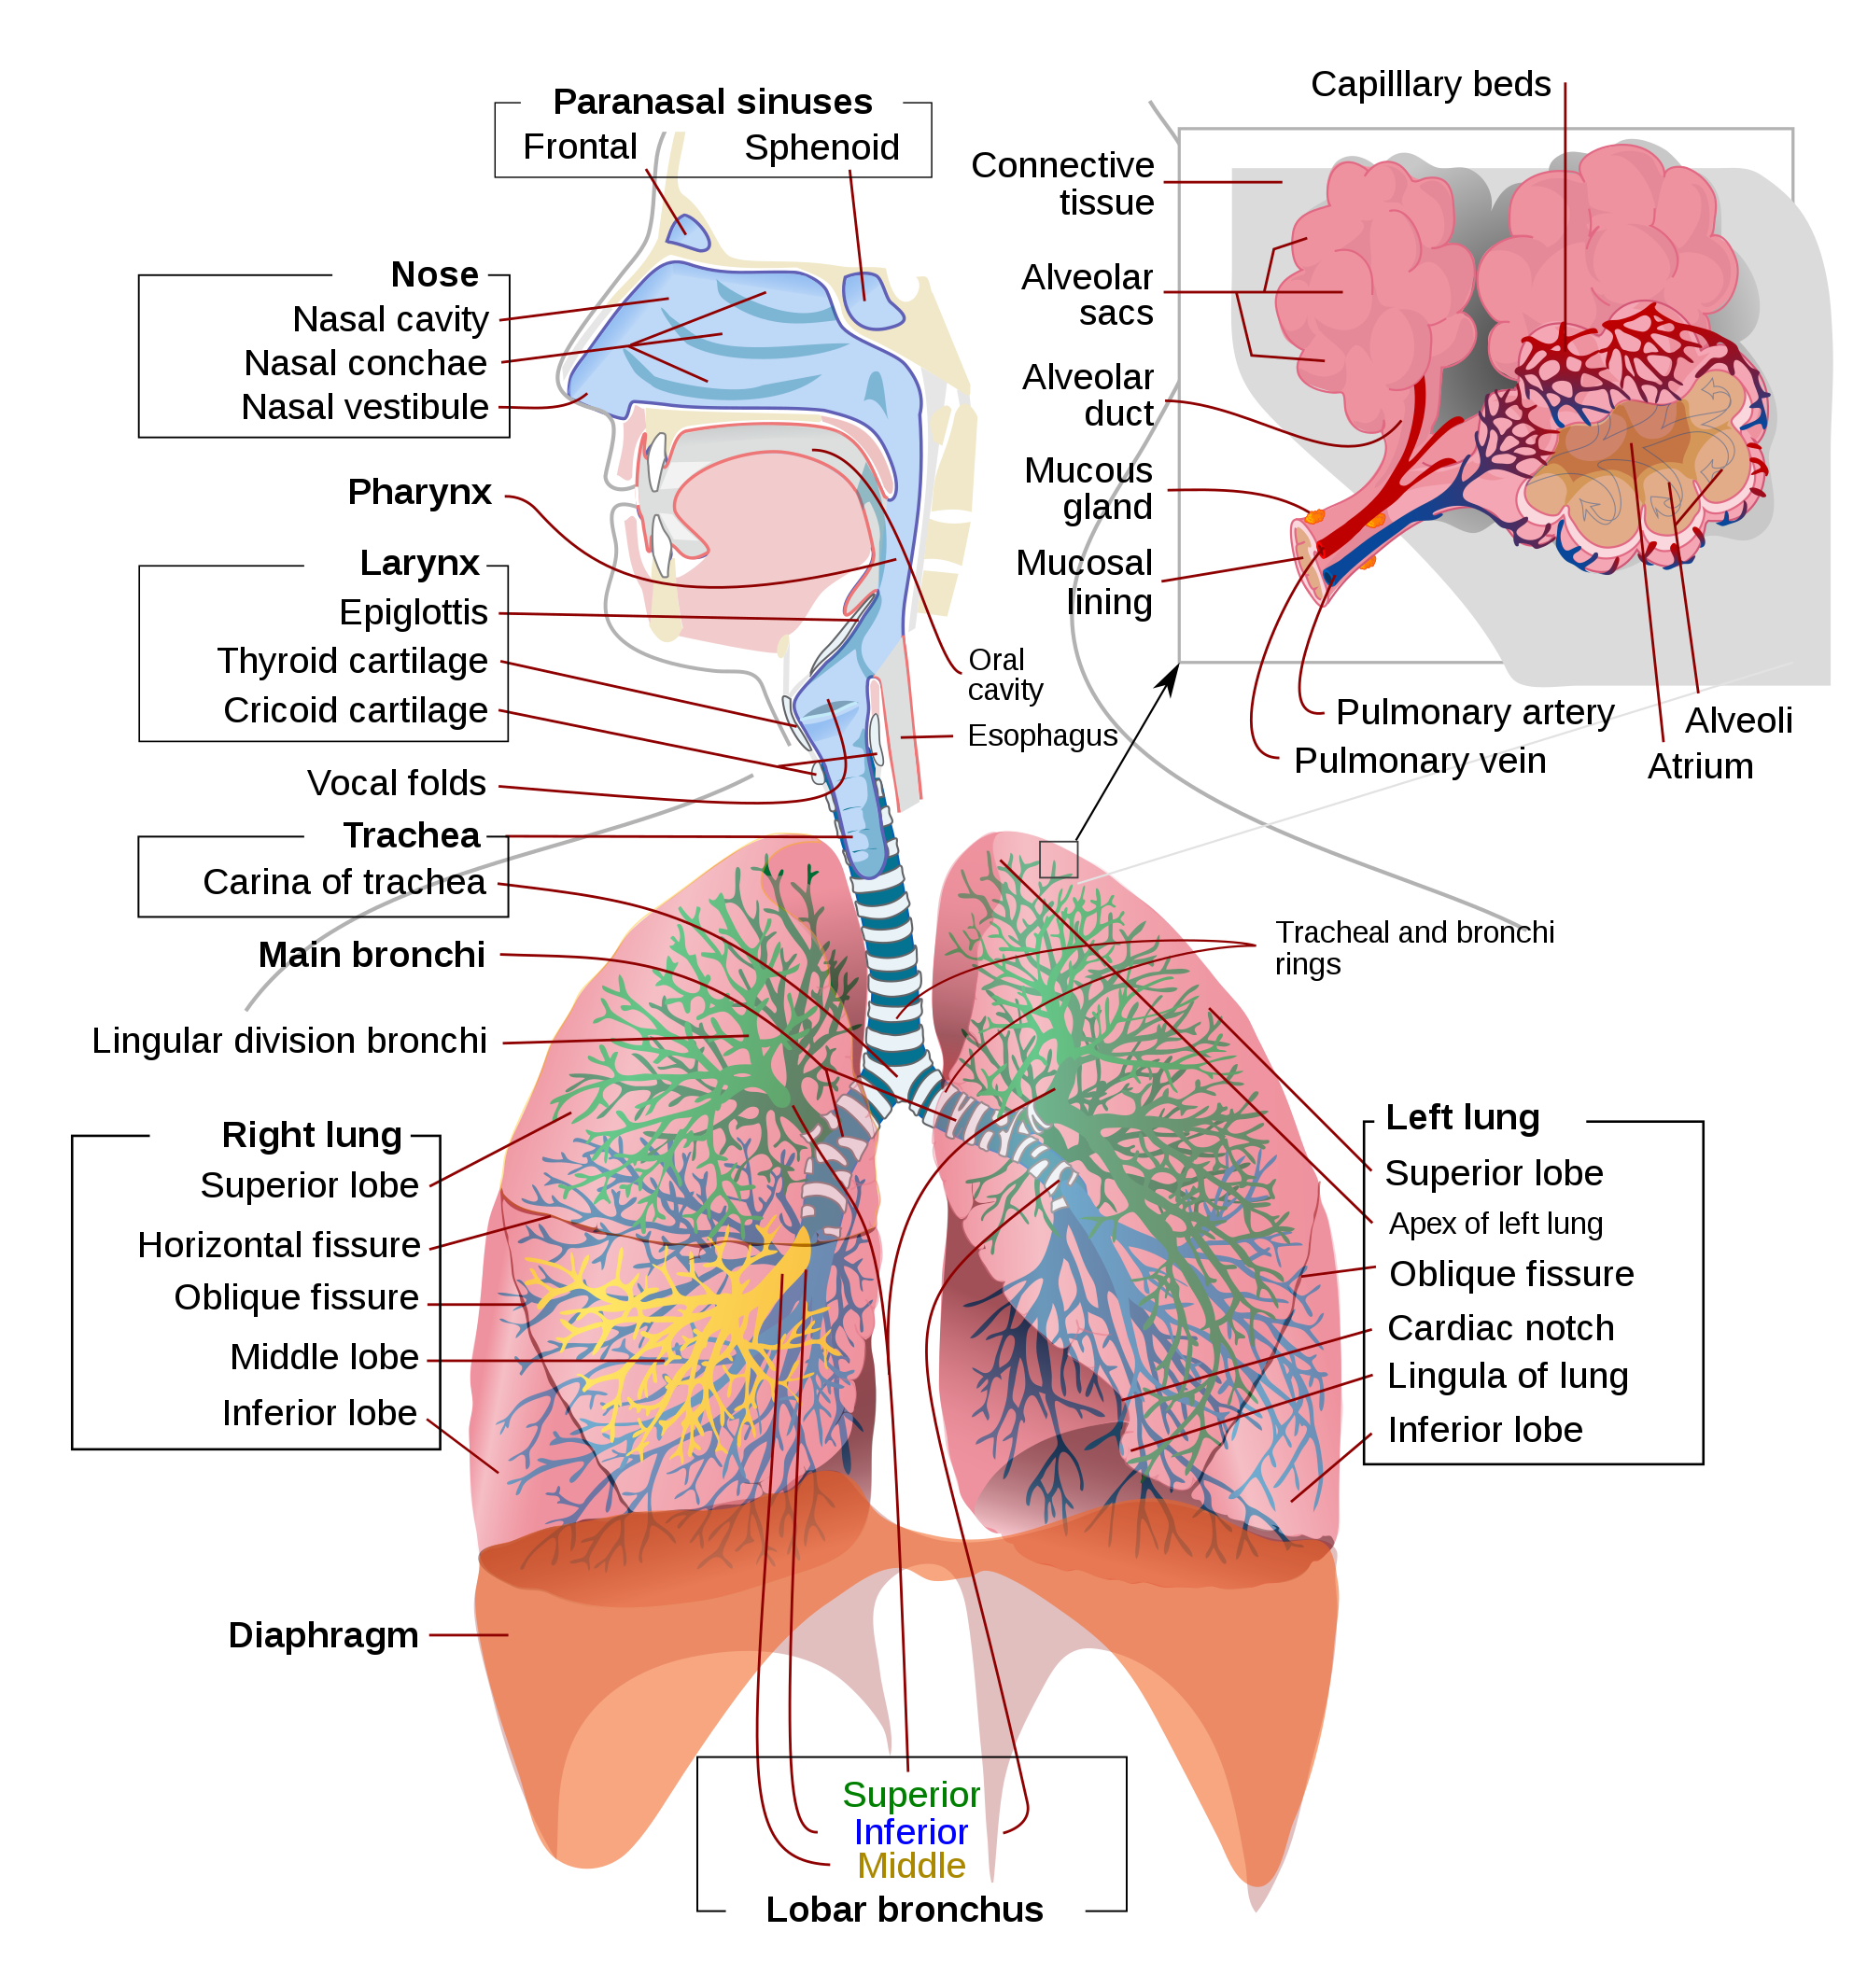
\includegraphics[width=0.7\linewidth]{./figures/respiratory/Respiratory_system_complete_en} 

}

\caption{\href{https://commons.wikimedia.org/wiki/File:Respiratory_system_complete_en.svg}{The respiratory system consists of the airways, the lungs, and the respiratory muscles that mediate the movement of air into and out of the body.}}\label{fig:respiratorysystem}
\end{figure}

The branching airways of the lower tract are often described as the respiratory tree or tracheobronchial tree. The intervals between successive branch points along the various branches of ``tree'' are often referred to as branching ``generations'', of which there are, in the adult human about 23. The earlier generations (approximately generations 0--16), consisting of the trachea and the bronchi, as well as the larger bronchioles which simply act as air conduits, bringing air to the respiratory bronchioles, alveolar ducts and alveoli (approximately generations 17--23), where gas exchange takes place. Bronchioles are defined as the small airways lacking any cartilagenous support.

The first bronchi to branch from the trachea are the right and left main bronchi. Second only in diameter to the trachea (1.8 cm), these bronchi (1 -1.4 cm in diameter) enter the lungs at each hilum, where they branch into narrower secondary bronchi known as lobar bronchi, and these branch into narrower tertiary bronchi known as segmental bronchi. Further divisions of the segmental bronchi (1 to 6 mm in diameter) are known as 4th order, 5th order, and 6th order segmental bronchi, or grouped together as subsegmental bronchi.

The alveoli are the dead end terminals of the ``tree'', meaning that any air that enters them has to exit via the same route. A system such as this creates dead space, a volume of air (about 150 ml in the adult human) that fills the airways after exhalation and is breathed back into the alveoli before environmental air reaches them. At the end of inhalation the airways are filled with environmental air, which is exhaled without coming in contact with the gas exchanger.



\begin{figure}

{\centering 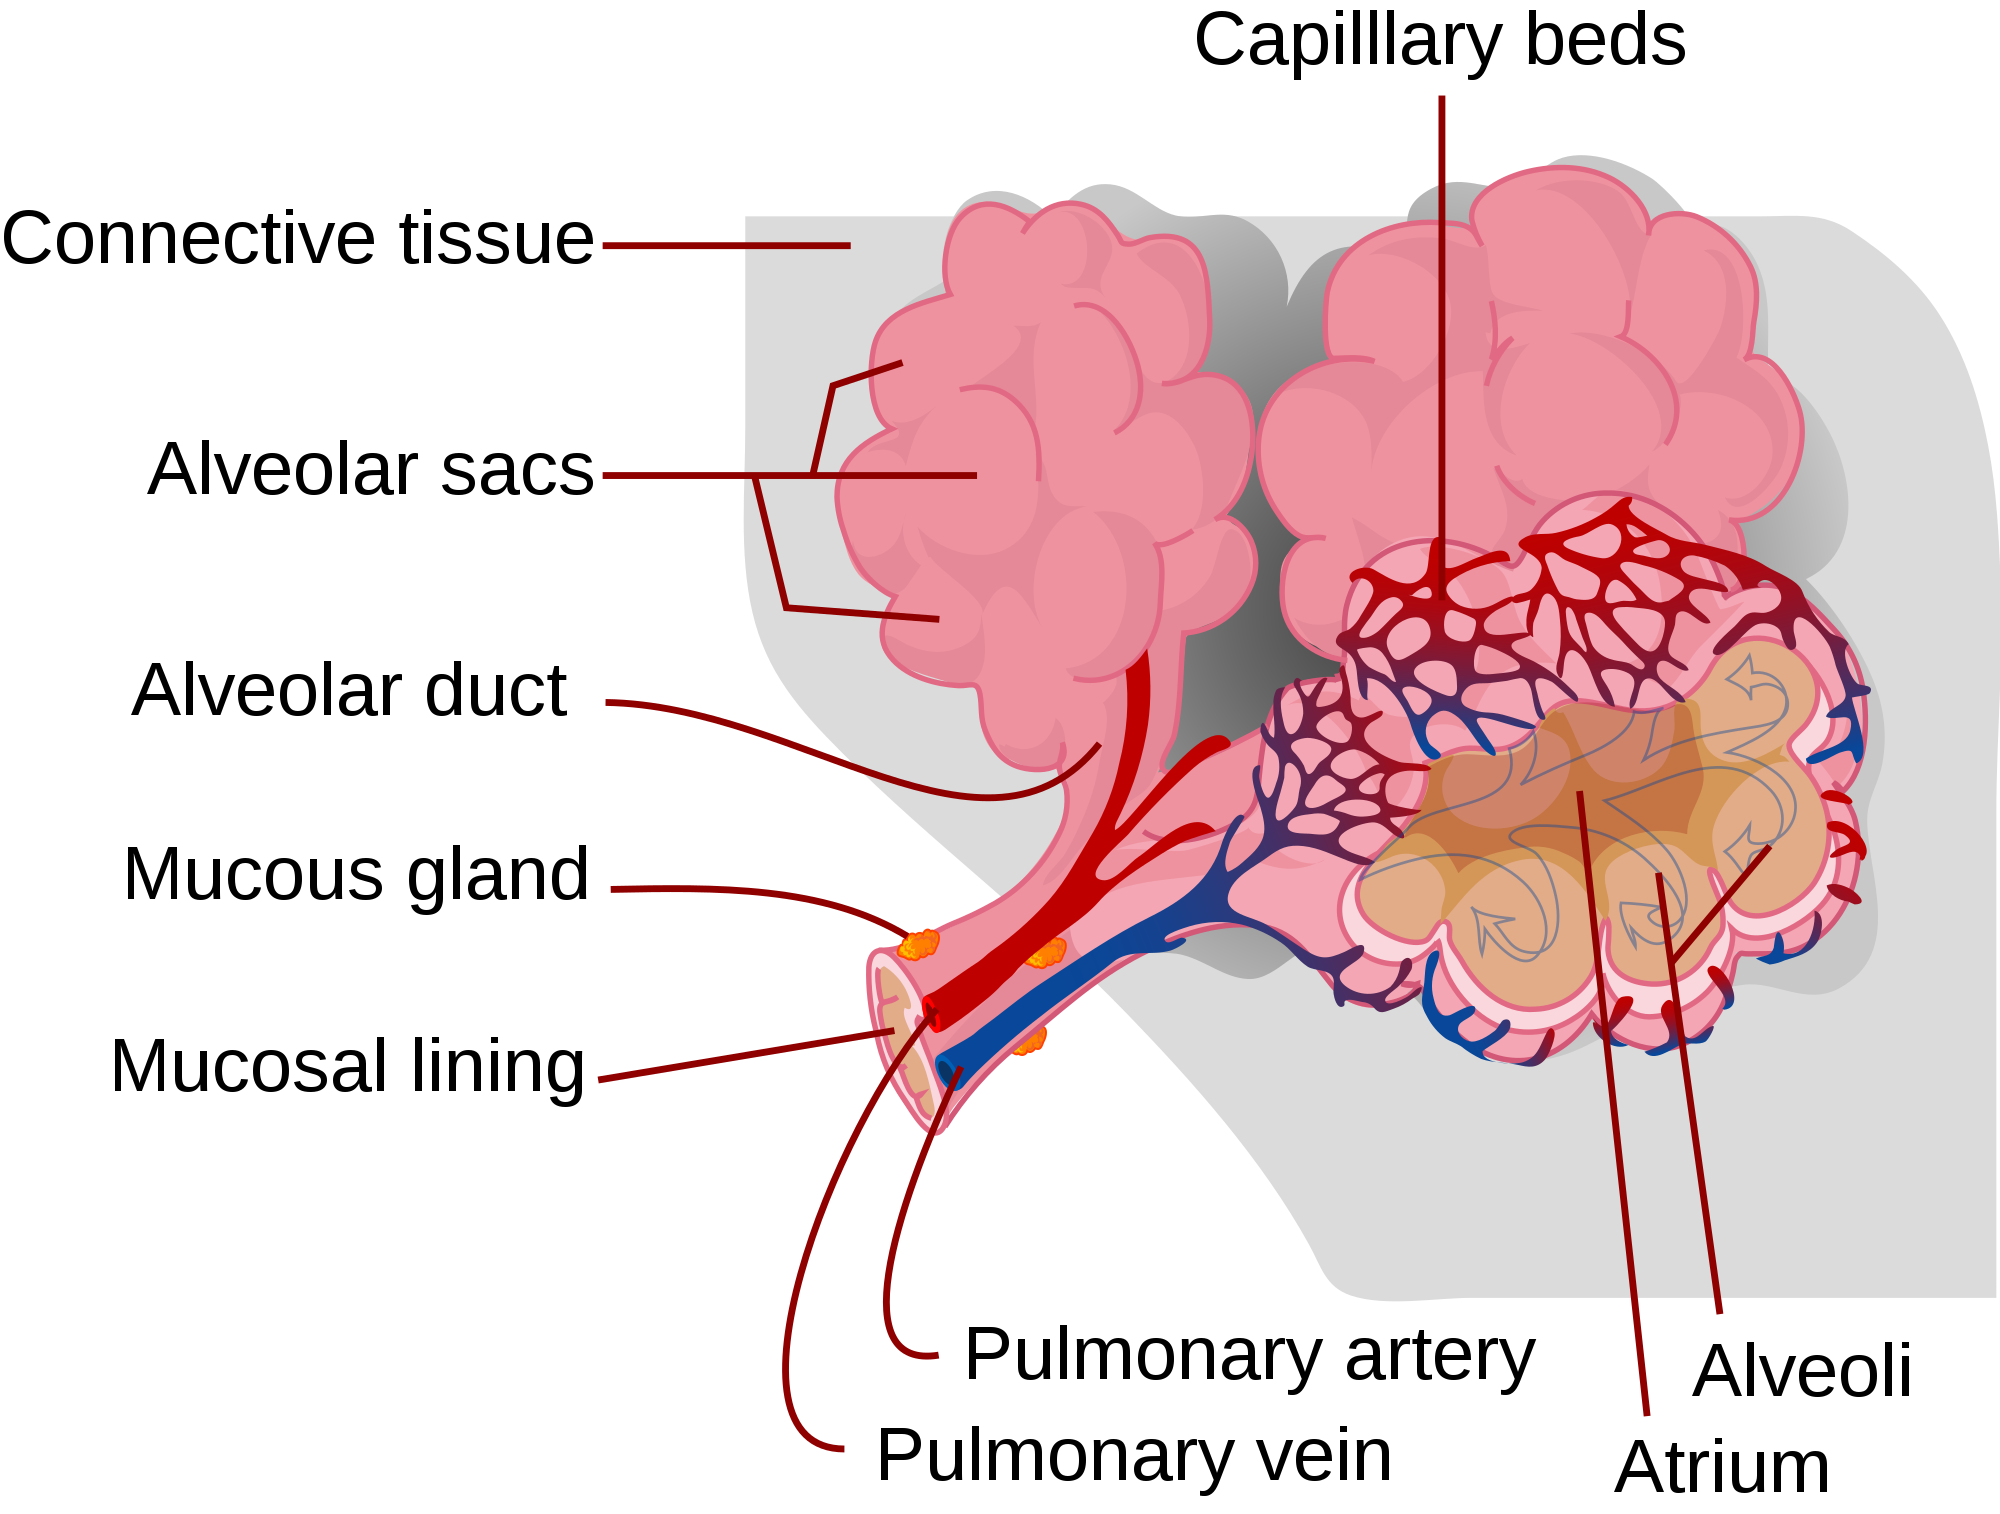
\includegraphics[width=0.7\linewidth]{./figures/respiratory/Alveolus diagram en} 

}

\caption{\href{https://upload.wikimedia.org/wikipedia/commons/4/46/Alveolus_diagram.svg}{Alveoli and their capillary networks.}}\label{fig:alveolusdiagram}
\end{figure}

The lungs expand and contract during the breathing cycle, drawing air in and out of the lungs. The volume of air moved in or out of the lungs under normal resting circumstances (the resting tidal volume of about 500 ml), and volumes moved during maximally forced inhalation and maximally forced exhalation are measured in humans by spirometry.



\begin{figure}

{\centering 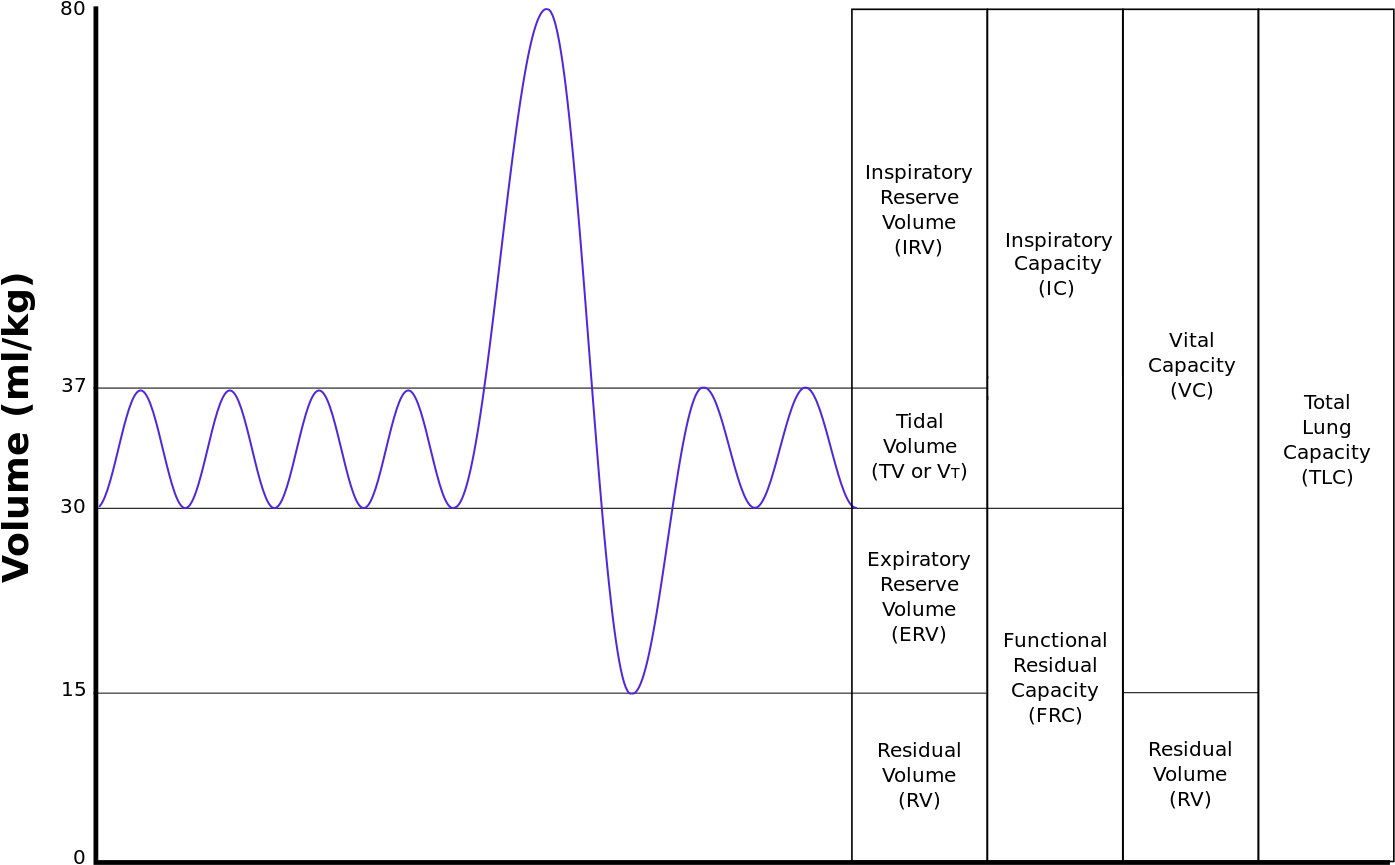
\includegraphics[width=0.7\linewidth]{./figures/respiratory/Lungvolumes_Updated} 

}

\caption{\href{https://commons.wikimedia.org/wiki/File:Lungvolumes_Updated.png}{Output of a `spirometer'. Upward movement of the graph, read from the left, indicates the intake of air; downward movements represent exhalation.}}\label{fig:spirometeroutput}
\end{figure}

Not all the air in the lungs can be expelled during maximally forced exhalation. This is the residual volume of about 1.0-1.5 liters which cannot be measured by spirometry. Volumes that include the residual volume (i.e.~functional residual capacity of about 2.5-3.0 liters, and total lung capacity of about 6 liters) can therefore also not be measured by spirometry. Their measurement requires special techniques.

The rates at which air is breathed in or out, either through the mouth or nose, or into or out of the alveoli are tabulated below, together with how they are calculated. The number of breath cycles per minute is known as the respiratory rate.

In mammals, inhalation at rest is primarily due to the contraction of the diaphragm. This is an upwardly domed sheet of muscle that separates the thoracic cavity from the abdominal cavity. When it contracts the sheet flattens, (i.e.~moves downwards as shown in Fig. 7) increasing the volume of the thoracic cavity. The contracting diaphragm pushes the abdominal organs downwards. But because the pelvic floor prevents the lowermost abdominal organs moving in that direction, the pliable abdominal contents cause the belly to bulge outwards to the front and sides, because the relaxed abdominal muscles do not resist this movement (Fig. 7). This entirely passive bulging (and shrinking during exhalation) of the abdomen during normal breathing is sometimes referred to as ``abdominal breathing'', although it is, in fact, ``diaphragmatic breathing'', which is not visible on the outside of the body. Mammals only use their abdominal muscles only during forceful exhalation (see Fig. 8, and discussion below). Never during any form of inhalation.

The enlargement of the thoracic cavity's vertical dimension by the contraction of the diaphragm, and its two horizontal dimensions by the lifting of the front and sides of the ribs, causes the intrathoracic pressure to fall. The lungs' interiors are open to the outside air, and being elastic, therefore expand to fill the increased space. The inflow of air into the lungs occurs via the respiratory airways. In health, these airways begin with the nose. It is possible to begin with the mouth, which is the backup breathing system. However, chronic mouth breathing leads to, or is a sign of, illness. They end in the microscopic dead-end sacs called alveoli) are always open, though the diameters of the various sections can be changed by the sympathetic and parasympathetic nervous systems. The alveolar air pressure is therefore always close to atmospheric air pressure (about 100 kPa at sea level) at rest, with the pressure gradients that cause air to move in and out of the lungs during breathing rarely exceeding 2--3 kPa.

During exhalation the diaphragm and intercostal muscles relax. This returns the chest and abdomen to a position determined by their anatomical elasticity. This is the ``resting mid-position'' of the thorax and abdomen when the lungs contain their functional residual capacity of air (the light blue area in the right hand illustration of Fig. 7), which in the adult human has a volume of about 2.5--3.0 liters. Resting exhalation lasts about twice as long as inhalation because the diaphragm relaxes passively more gently than it contracts actively during inhalation.

The volume of air that moves in or out (at the nose or mouth) during a single breathing cycle is called the tidal volume. In a resting adult human it is about 500 ml per breath. At the end of exhalation the airways contain about 150 ml of alveolar air which is the first air that is breathed back into the alveoli during inhalation. This volume air that is breathed out of the alveoli and back in again is known as dead space ventilation, which has the consequence that of the 500 ml breathed into the alveoli with each breath only 350 ml (500 ml - 150 ml = 350 ml) is fresh warm and moistened air. Since this 350 ml of fresh air is thoroughly mixed and diluted by the air that remains in the alveoli after normal exhalation (i.e.~the functional residual capacity of about 2.5--3.0 liters), it is clear that the composition of the alveolar air changes very little during the breathing cycle (see Fig. 9). The oxygen tension (or partial pressure) remains close to 13-14 kPa (about 100 mm Hg), and that of carbon dioxide very close to 5.3 kPa (or 40 mm Hg). This contrasts with composition of the dry outside air at sea level, where the partial pressure of oxygen is 21 kPa (or 160 mm Hg) and that of carbon dioxide 0.04 kPa (or 0.3 mmHg).

During heavy breathing (hyperpnea), as, for instance, during exercise, inhalation is brought about by a more powerful and greater excursion of the contracting diaphragm than at rest. In addition the ``accessory muscles of inhalation'' exaggerate the actions of the intercostal muscles (Fig. 8). These accessory muscles of inhalation are muscles that extend from the cervical vertebrae and base of the skull to the upper ribs and sternum, sometimes through an intermediary attachment to the clavicles. When they contract the rib cage's internal volume is increased to a far greater extent than can be achieved by contraction of the intercostal muscles alone. Seen from outside the body the lifting of the clavicles during strenuous or labored inhalation is sometimes called clavicular breathing, seen especially during asthma attacks and in people with chronic obstructive pulmonary disease.

During heavy breathing, exhalation is caused by relaxation of all the muscles of inhalation. But now, the abdominal muscles, instead of remaining relaxed (as they do at rest), contract forcibly pulling the lower edges of the rib cage downwards (front and sides). This not only drastically decreases the size of the rib cage, but also pushes the abdominal organs upwards against the diaphragm which consequently bulges deeply into the thorax. The end-exhalatory lung volume is now well below the resting mid-position and contains far less air than the resting ``functional residual capacity''. However, in a normal mammal, the lungs cannot be emptied completely. In an adult human there is always still at least 1 liter of residual air left in the lungs after maximum exhalation.

The automatic rhythmical breathing in and out, can be interrupted by coughing, sneezing (forms of very forceful exhalation), by the expression of a wide range of emotions (laughing, sighing, crying out in pain, exasperated intakes of breath) and by such voluntary acts as speech, singing, whistling and the playing of wind instruments. All of these actions rely on the muscles described above, and their effects on the movement of air in and out of the lungs.

Although not a form of breathing, the Valsalva maneuver involves the respiratory muscles. It is, in fact, a very forceful exhalatory effort against a tightly closed glottis, so that no air can escape from the lungs. Instead abdominal contents are evacuated in the opposite direction, through orifices in the pelvic floor. The abdominal muscles contract very powerfully, causing the pressure inside the abdomen and thorax to rise to extremely high levels. The Valsalva maneuver can be carried out voluntarily, but is more generally a reflex elicited when attempting to empty the abdomen during, for instance, difficult defecation, or during childbirth. Breathing ceases during this maneuver.

\hypertarget{gas-exchange}{%
\section{Gas Exchange}\label{gas-exchange}}

The primary purpose of the respiratory system is the equilibration of the partial pressures of the respiratory gases in the alveolar air with those in the pulmonary capillary blood. This process occurs by simple diffusion, across a very thin membrane (known as the blood--air barrier), which forms the walls of the pulmonary alveoli (Figure \ref{fig:alveolarwall}). It consisting of the alveolar epithelial cells, their basement membranes and the endothelial cells of the alveolar capillaries (Figure \ref{fig:alveolarwall}). This blood gas barrier is extremely thin (in humans, on average, 2.2 μm thick). It is folded into about 300 million small air sacs called alveoli (each between 75 and 300 µm in diameter) branching off from the respiratory bronchioles in the lungs, thus providing an extremely large surface area (approximately 145 m2) for gas exchange to occur.

(ref:alve)\href{https://upload.wikimedia.org/wikipedia/commons/c/c8/Alveolar_wall.jpg}{A histological cross-section through an alveolar wall showing the layers through which the gases have to move between the blood plasma and the alveolar air. The dark blue objects are the nuclei of the capillary endothelial and alveolar type I epithelial cells (or type 1 pneumocytes). The two red objects labeled ``RBC'' are red blood cells in the pulmonary capillary blood.}

\begin{figure}

{\centering 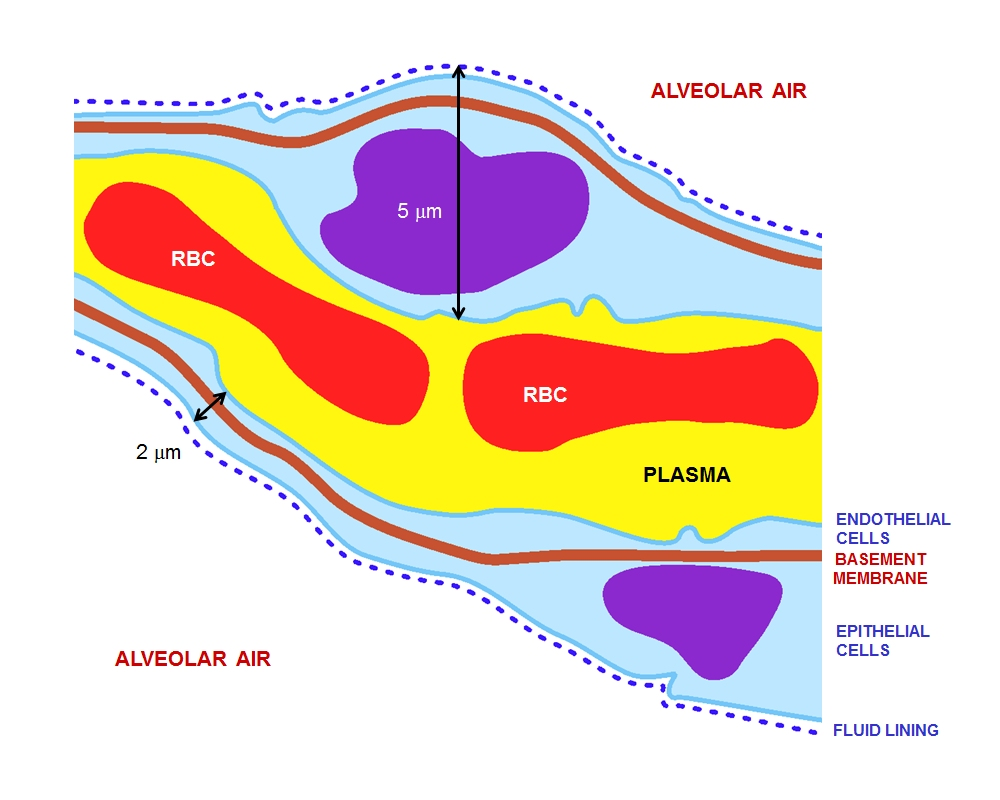
\includegraphics[width=0.7\linewidth]{./figures/respiratory/Alveolar_wall} 

}

\caption{(ref:alve)}\label{fig:alveolarwall}
\end{figure}

The air contained within the alveoli has a semi-permanent volume of about 2.5-3.0 liters which completely surrounds the alveolar capillary blood. This ensures that equilibration of the partial pressures of the gases in the two compartments is very efficient and occurs very quickly. The blood leaving the alveolar capillaries and is eventually distributed throughout the body therefore has a partial pressure of oxygen of 13-14 kPa (100 mmHg), and a partial pressure of carbon dioxide of 5.3 kPa (40 mmHg) (i.e.~the same as the oxygen and carbon dioxide gas tensions as in the alveoli). As mentioned in the section above, the corresponding partial pressures of oxygen and carbon dioxide in the ambient (dry) air at sea level are 21 kPa (160 mmHg) and 0.04 kPa (0.3 mmHg) respectively.

This marked difference between the composition of the alveolar air and that of the ambient air can be maintained because the functional residual capacity is contained in dead-end sacs connected to the outside air by fairly narrow and relatively long tubes (the airways: nose, pharynx, larynx, trachea, bronchi and their branches down to the bronchioles), through which the air has to be breathed both in and out (i.e.~there is no unidirectional through-flow as there is in the bird lung). This typical mammalian anatomy combined with the fact that the lungs are not emptied and re-inflated with each breath (leaving a substantial volume of air, of about 2.5-3.0 liters, in the alveoli after exhalation), ensures that the composition of the alveolar air is only minimally disturbed when the 350 ml of fresh air is mixed into it with each inhalation. Thus the animal is provided with a very special ``portable atmosphere'', whose composition differs significantly from the present-day ambient air. It is this portable atmosphere (the functional residual capacity) to which the blood and therefore the body tissues are exposed -- not to the outside air.

The resulting arterial partial pressures of oxygen and carbon dioxide are homeostatically controlled. A rise in the arterial partial pressure of CO\textsubscript{2}) and, to a lesser extent, a fall in the arterial partial pressure of O\textsubscript{2}), will reflexly cause deeper and faster breathing till the blood gas tensions in the lungs, and therefore the arterial blood, return to normal. The converse happens when the carbon dioxide tension falls, or, again to a lesser extent, the oxygen tension rises: the rate and depth of breathing are reduced till blood gas normality is restored.

Since the blood arriving in the alveolar capillaries has a partial pressure of O\textsubscript{2}) of, on average, 6 kPa (45 mmHg), while the pressure in the alveolar air is 13-14 kPa (100 mmHg), there will be a net diffusion of oxygen into the capillary blood, changing the composition of the 3 liters of alveolar air slightly. Similarly, since the blood arriving in the alveolar capillaries has a partial pressure of CO\textsubscript{2}) of also about 6 kPa (45 mmHg), whereas that of the alveolar air is 5.3 kPa (40 mmHg), there is a net movement of carbon dioxide out of the capillaries into the alveoli. The changes brought about by these net flows of individual gases into and out of the alveolar air necessitate the replacement of about 15\% of the alveolar air with ambient air every 5 seconds or so. This is very tightly controlled by the monitoring of the arterial blood gases (which accurately reflect composition of the alveolar air) by the aortic and carotid bodies, as well as by the blood gas and pH sensor on the anterior surface of the medulla oblongata in the brain. There are also oxygen and carbon dioxide sensors in the lungs, but they primarily determine the diameters of the bronchioles and pulmonary capillaries, and are therefore responsible for directing the flow of air and blood to different parts of the lungs.



\begin{figure}

{\centering 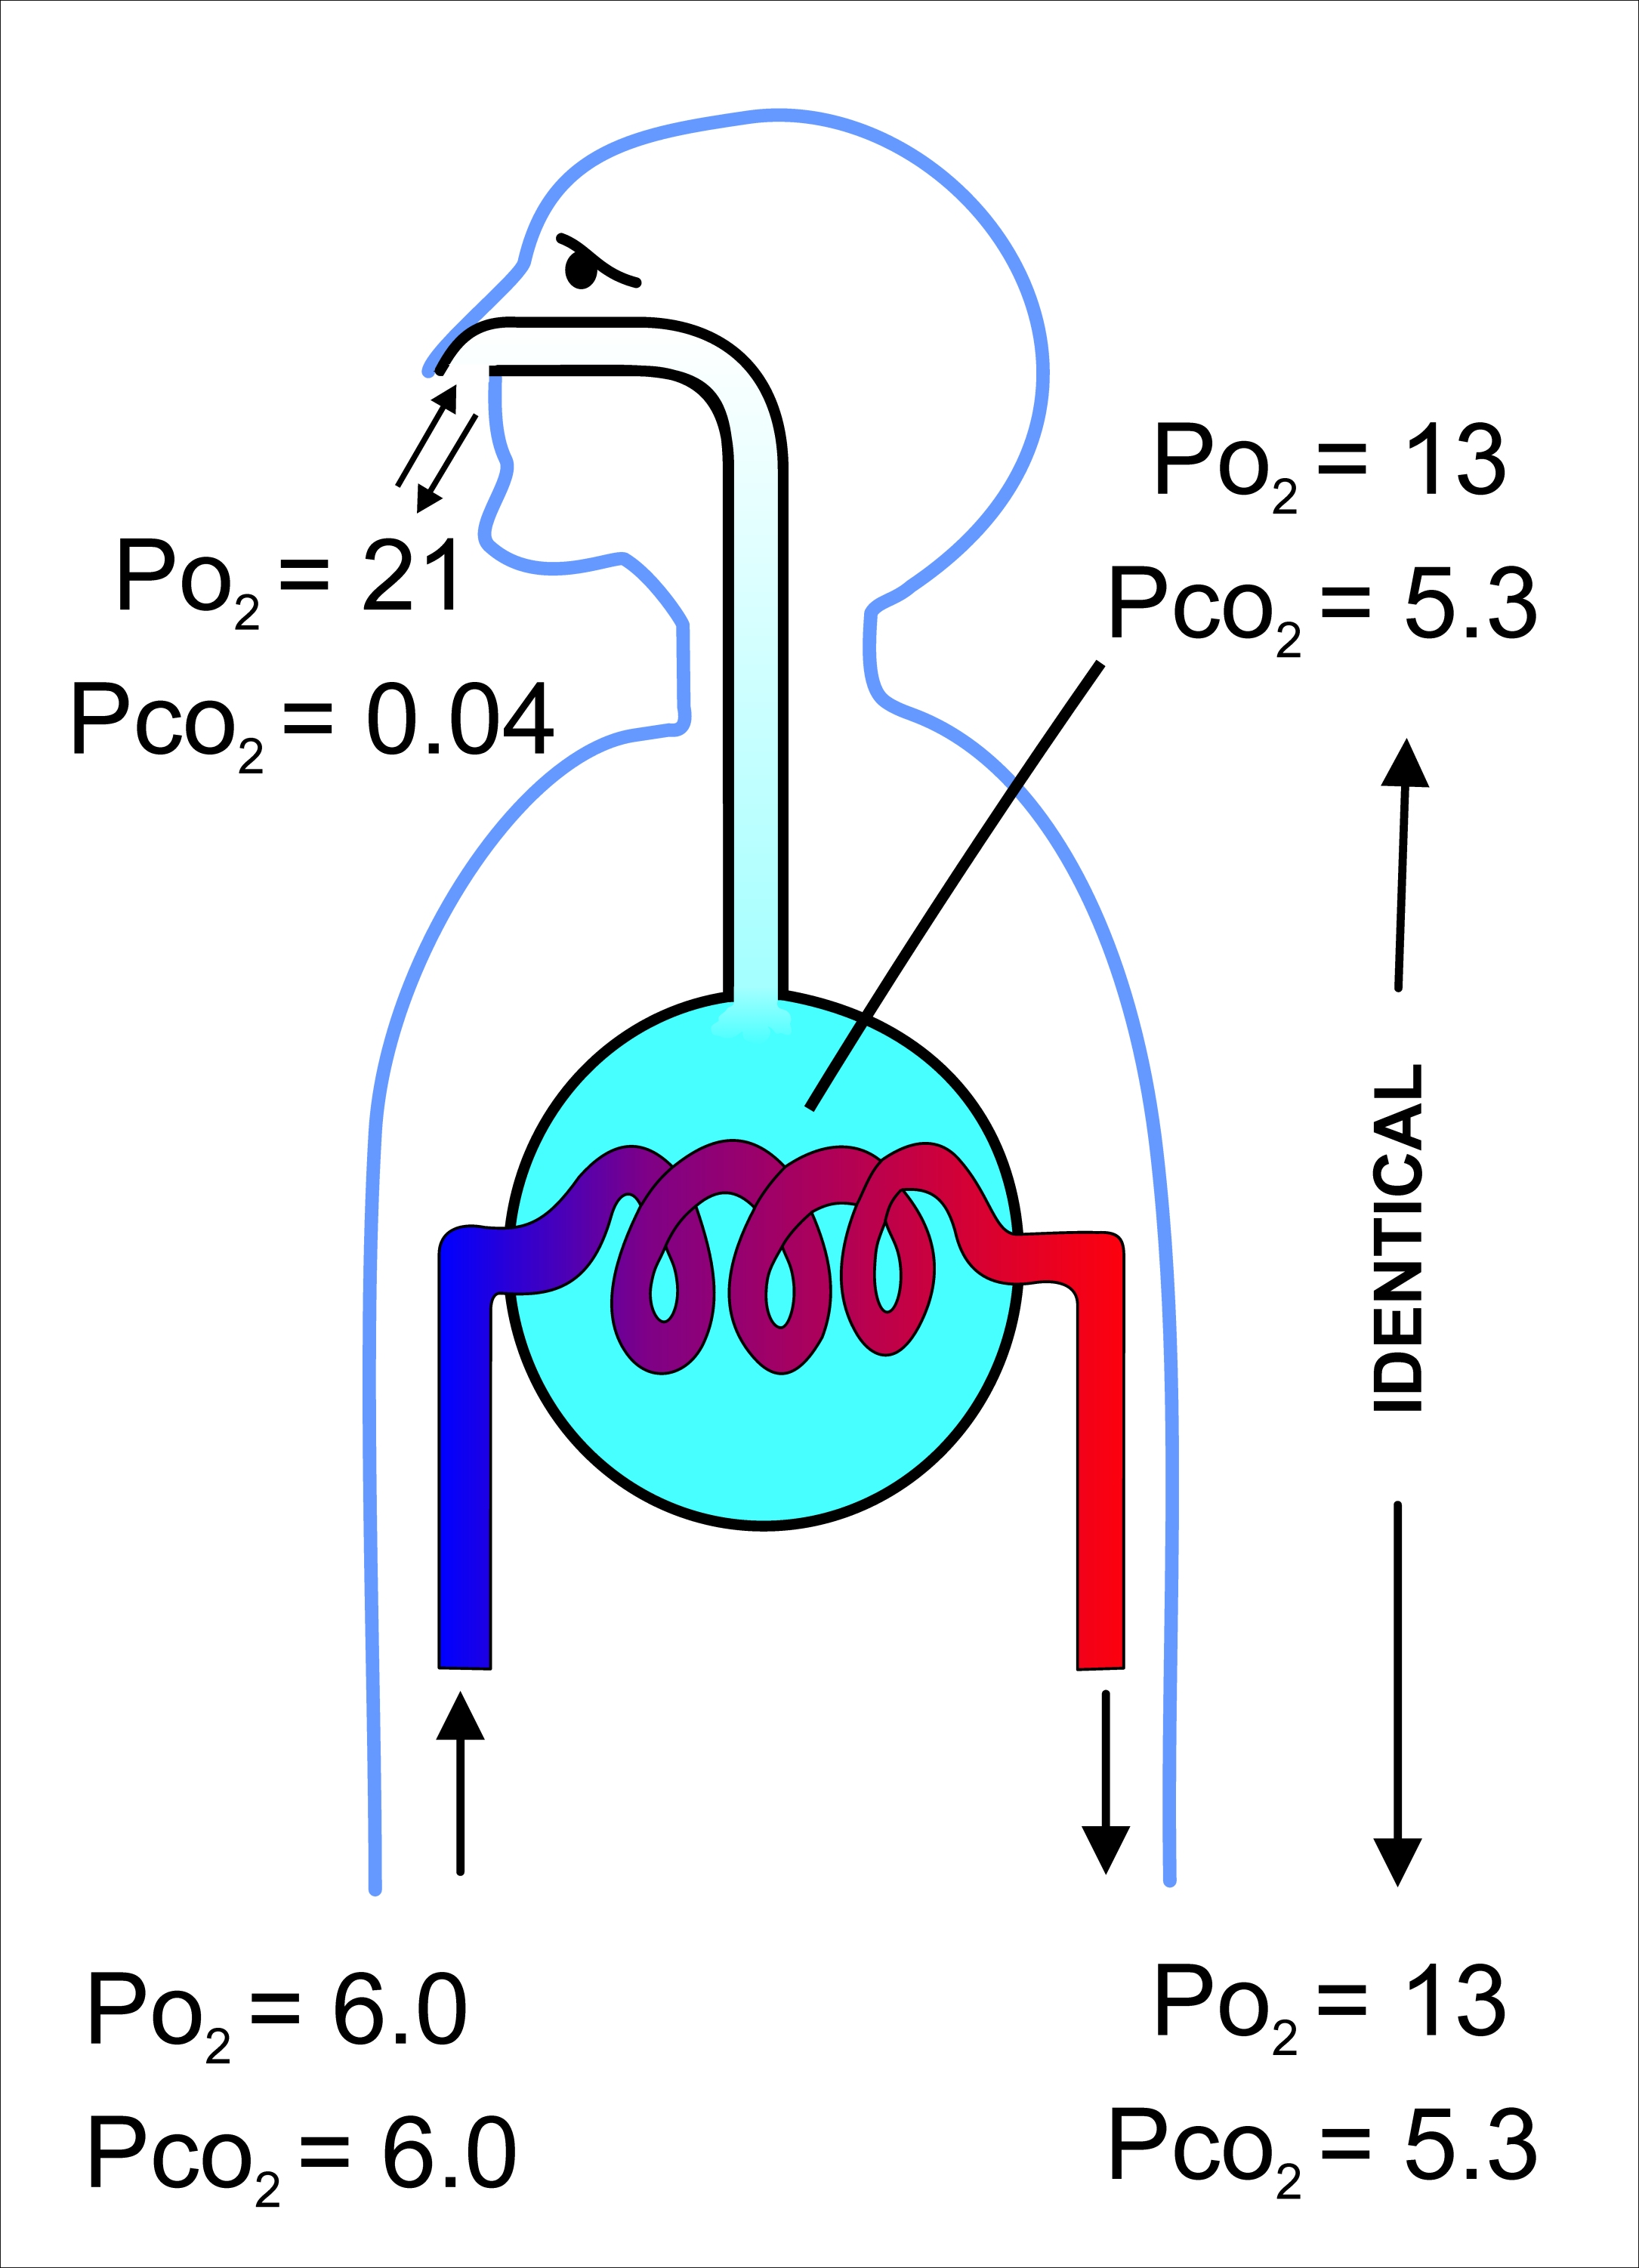
\includegraphics[width=0.7\linewidth]{./figures/respiratory/Gas_exchange} 

}

\caption{\href{https://commons.wikimedia.org/wiki/File:Gas_exchange.jpg}{A highly diagrammatic illustration of the process of gas exchange in the mammalian lungs, emphasizing the differences between the gas compositions of the ambient air, the alveolar air (light blue) with which the pulmonary capillary blood equilibrates, and the blood gas tensions in the pulmonary arterial (blue blood entering the lung on the left) and venous blood (red blood leaving the lung on the right). All the gas tensions are in kPa. To convert to mm Hg, multiply by 7.5.}}\label{fig:gasexchange}
\end{figure}

It is only as a result of accurately maintaining the composition of the 3 liters of alveolar air that with each breath some carbon dioxide is discharged into the atmosphere and some oxygen is taken up from the outside air. If more carbon dioxide than usual has been lost by a short period of hyperventilation, respiration will be slowed down or halted until the alveolar partial pressure of carbon dioxide has returned to 5.3 kPa (40 mmHg). It is therefore strictly speaking untrue that the primary function of the respiratory system is to rid the body of carbon dioxide ``waste''. The carbon dioxide that is breathed out with each breath could probably be more correctly be seen as a byproduct of the body's extracellular fluid carbon dioxide and pH homeostats



\begin{figure}

{\centering 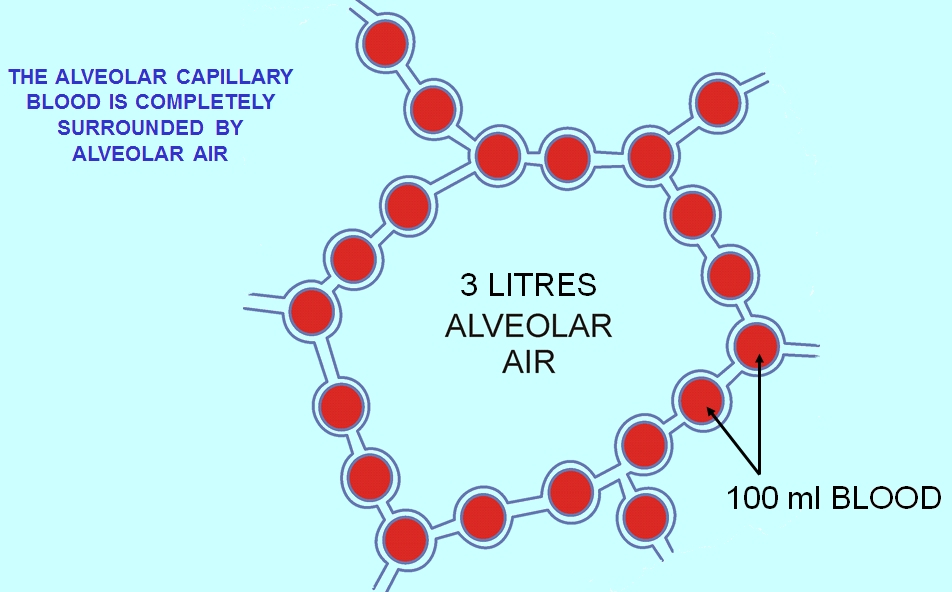
\includegraphics[width=0.7\linewidth]{./figures/respiratory/Alveolus} 

}

\caption{\href{https://commons.wikimedia.org/wiki/File:Alveolus.jpg}{A diagrammatic histological cross-section through a portion of lung tissue showing a normally inflated alveolus (at the end of a normal exhalation), and its walls containing the pulmonary capillaries (shown in cross-section). This illustrates how the pulmonary capillary blood is completely surrounded by alveolar air. In a normal human lung all the alveoli together contain about 3 liters of alveolar air. All the pulmonary capillaries contain about 100 ml blood.}}\label{fig:alveolarair}
\end{figure}

If these homeostats are compromised, then a respiratory acidosis, or a respiratory alkalosis will occur. In the long run these can be compensated by renal adjustments to the H+ and HCO3− concentrations in the plasma; but since this takes time, the hyperventilation syndrome can, for instance, occur when agitation or anxiety cause a person to breathe fast and deeply thus causing a distressing respiratory alkalosis through the blowing off of too much CO\textsubscript{2}) from the blood into the outside air.

Oxygen has a very low solubility in water, and is therefore carried in the blood loosely combined with hemoglobin. The oxygen is held on the hemoglobin by four ferrous iron-containing heme groups per hemoglobin molecule. When all the heme groups carry one O\textsubscript{2}) molecule each the blood is said to be ``saturated'' with oxygen, and no further increase in the partial pressure of oxygen will meaningfully increase the oxygen concentration of the blood. Most of the carbon dioxide in the blood is carried as bicarbonate ions (HCO3−) in the plasma. However the conversion of dissolved CO\textsubscript{2}) into HCO3− (through the addition of water) is too slow for the rate at which the blood circulates through the tissues on the one hand, and through alveolar capillaries on the other. The reaction is therefore catalyzed by carbonic anhydrase, an enzyme inside the red blood cells. The reaction can go in both directions depending on the prevailing partial pressure of CO\textsubscript{2}). A small amount of carbon dioxide is carried on the protein portion of the hemoglobin molecules as carbamino groups. The total concentration of carbon dioxide (in the form of bicarbonate ions, dissolved CO\textsubscript{2}), and carbamino groups) in arterial blood (i.e.~after it has equilibrated with the alveolar air) is about 26 mM (or 58 ml/100 ml), compared to the concentration of oxygen in saturated arterial blood of about 9 mM (or 20 ml/100 ml blood).

\hypertarget{control-of-ventilation}{%
\section{Control of Ventilation}\label{control-of-ventilation}}

Ventilation of the lungs in mammals occurs via the respiratory centers in the medulla oblongata and the pons of the brainstem. These areas form a series of neural pathways which receive information about the partial pressures of oxygen and carbon dioxide in the arterial blood. This information determines the average rate of ventilation of the alveoli of the lungs, to keep these pressures constant. The respiratory center does so via motor nerves which activate the diaphragm and other muscles of respiration.

The breathing rate increases when the partial pressure of carbon dioxide in the blood increases. This is detected by central blood gas chemoreceptors on the anterior surface of the medulla oblongata. The aortic and carotid bodies, are the peripheral blood gas chemoreceptors which are particularly sensitive to the arterial partial pressure of O\textsubscript{2}) though they also respond, but less strongly, to the partial pressure of CO\textsubscript{2}). At sea level, under normal circumstances, the breathing rate and depth, is determined primarily by the arterial partial pressure of carbon dioxide rather than by the arterial partial pressure of oxygen, which is allowed to vary within a fairly wide range before the respiratory centers in the medulla oblongata and pons respond to it to change the rate and depth of breathing.

Exercise increases the breathing rate due to the extra carbon dioxide produced by the enhanced metabolism of the exercising muscles. In addition passive movements of the limbs also reflexively produce an increase in the breathing rate.

Information received from stretch receptors in the lungs limits tidal volume (the depth of inhalation and exhalation).

The respiratory system of birds differs significantly from that found in mammals. Firstly, they have rigid lungs which do not expand and contract during the breathing cycle. Instead an extensive system of air sacs (Fig. 15) distributed throughout their bodies act as the bellows drawing environmental air into the sacs, and expelling the spent air after it has passed through the lungs. Birds also do not have diaphragms or pleural cavities.

Bird lungs are smaller than those in mammals of comparable size, but the air sacs account for 15\% of the total body volume, compared to the 7\% devoted to the alveoli which act as the bellows in mammals.

Inhalation and exhalation are brought about by alternately increasing and decreasing the volume of the entire thoraco-abdominal cavity (or coelom) using both their abdominal and costal muscles. During inhalation the muscles attached to the vertebral ribs (Fig. 17) contract angling them forwards and outwards. This pushes the sternal ribs, to which they are attached at almost right angles, downwards and forwards, taking the sternum (with its prominent keel) in the same direction (Fig. 17). This increases both the vertical and transverse diameters of thoracic portion of the trunk. The forward and downward movement of, particularly, the posterior end of the sternum pulls the abdominal wall downwards, increasing the volume of that region of the trunk as well. The increase in volume of the entire trunk cavity reduces the air pressure in all the thoraco-abdominal air sacs, causing them to fill with air as described below.

During exhalation the external oblique muscle which is attached to the sternum and vertebral ribs anteriorly, and to the pelvis (pubis and ilium in Fig. 17) posteriorly (forming part of the abdominal wall) reverses the inhalatory movement, while compressing the abdominal contents, thus increasing the pressure in all the air sacs. Air is therefore expelled from the respiratory system in the act of exhalation.

During inhalation air enters the trachea via the nostrils and mouth, and continues to just beyond the syrinx at which point the trachea branches into two primary bronchi, going to the two lungs (Fig. 16). The primary bronchi enter the lungs to become the intrapulmonary bronchi, which give off a set of parallel branches called ventrobronchi and, a little further on, an equivalent set of dorsobronchi (Fig. 16). The ends of the intrapulmonary bronchi discharge air into the posterior air sacs at the caudal end of the bird. Each pair of dorso-ventrobronchi is connected by a large number of parallel microscopic air capillaries (or parabronchi) where gas exchange occurs (Fig. 16). As the bird inhales, tracheal air flows through the intrapulmonary bronchi into the posterior air sacs, as well as into the dorsobronchi, but not into the ventrobronchi (Fig. 18). This is due to the bronchial architecture which directs the inhaled air away from the openings of the ventrobronchi, into the continuation of the intrapulmonary bronchus towards the dorsobronchi and posterior air sacs. From the dorsobronchi the inhaled air flows through the parabronchi (and therefore the gas exchanger) to the ventrobronchi from where the air can only escape into the expanding anterior air sacs. So, during inhalation, both the posterior and anterior air sacs expand, the posterior air sacs filling with fresh inhaled air, while the anterior air sacs fill with ``spent'' (oxygen-poor) air that has just passed through the lungs.

During exhalation the pressure in the posterior air sacs (which were filled with fresh air during inhalation) increases due to the contraction of the oblique muscle described above. The aerodynamics of the interconnecting openings from the posterior air sacs to the dorsobronchi and intrapulmonary bronchi ensures that the air leaves these sacs in the direction of the lungs (via the dorsobronchi), rather than returning down the intrapulmonary bronchi (Fig. 18). From the dorsobronchi the fresh air from the posterior air sacs flows through the parabronchi (in the same direction as occurred during inhalation) into ventrobronchi. The air passages connecting the ventrobronchi and anterior air sacs to the intrapulmonary bronchi direct the ``spent'', oxygen poor air from these two organs to the trachea from where it escapes to the exterior. Oxygenated air therefore flows constantly (during the entire breathing cycle) in a single direction through the parabronchi.

The blood flow through the bird lung is at right angles to the flow of air through the parabronchi, forming a cross-current flow exchange system (Fig. 19). The partial pressure of oxygen in the parabronchi declines along their lengths as O\textsubscript{2}) diffuses into the blood. The blood capillaries leaving the exchanger near the entrance of airflow take up more O\textsubscript{2}) than do the capillaries leaving near the exit end of the parabronchi. When the contents of all capillaries mix, the final partial pressure of oxygen of the mixed pulmonary venous blood is higher than that of the exhaled air, but is nevertheless less than half that of the inhaled air, thus achieving roughly the same systemic arterial blood partial pressure of oxygen as mammals do with their bellows-type lungs.

The trachea is an area of dead space: the oxygen-poor air it contains at the end of exhalation is the first air to re-enter the posterior air sacs and lungs. In comparison to the mammalian respiratory tract, the dead space volume in a bird is, on average, 4.5 times greater than it is in mammals of the same size. Birds with long necks will inevitably have long tracheae, and must therefore take deeper breaths than mammals do to make allowances for their greater dead space volumes. In some birds (e.g.~the whooper swan, Cygnus cygnus, the white spoonbill, Platalea leucorodia, the whooping crane, Grus americana, and the helmeted curassow, Pauxi pauxi) the trachea, which some cranes can be 1.5 m long, is coiled back and forth within the body, drastically increasing the dead space ventilation. The purpose of this extraordinary feature is unknown.

\hypertarget{the-respiratory-system-of-birds}{%
\section{The Respiratory System of Birds}\label{the-respiratory-system-of-birds}}

Due to the high metabolic rate required for flight, birds have a high oxygen demand. Their highly effective respiratory system helps them meet that demand.

Although birds have lungs, theirs are fairly rigid structures that do not expand and contract as they do in mammals, reptiles and many amphibians. Instead, the structures that act as the bellows that ventilate the lungs are the air sacs, which are distributed throughout much of the birds' bodies. The airsacs move air unidirectionally through the parabronchi of the rigid lungs. Although bird lungs are smaller than those of mammals of comparable size, the air sacs account for 15\% of the total body volume, whereas in mammals, the alveoli, which act as the bellows, constitute only 7\% of the total body volume. The walls of the air sacs do not have a good blood supply and so do not play a direct role in gas exchange.

Birds lack a diaphragm, and therefore use their intercostal and abdominal muscles to expand and contract their entire thoraco-abdominal cavities, thus rhythmically changing the volumes of all their air sacs in unison (illustration on the right). The active phase of respiration in birds is exhalation, requiring contraction of their muscles of respiration. Relaxation of these muscles causes inhalation.

Three distinct sets of organs perform respiration --- the anterior air sacs (interclavicular, cervicals, and anterior thoracics), the lungs, and the posterior air sacs (posterior thoracics and abdominals). Typically there are nine air sacs within the system; however, that number can range between seven and twelve, depending on the species of bird. Passerines possess seven air sacs, as the clavicular air sacs may interconnect or be fused with the anterior thoracic sacs.



\begin{figure}

{\centering 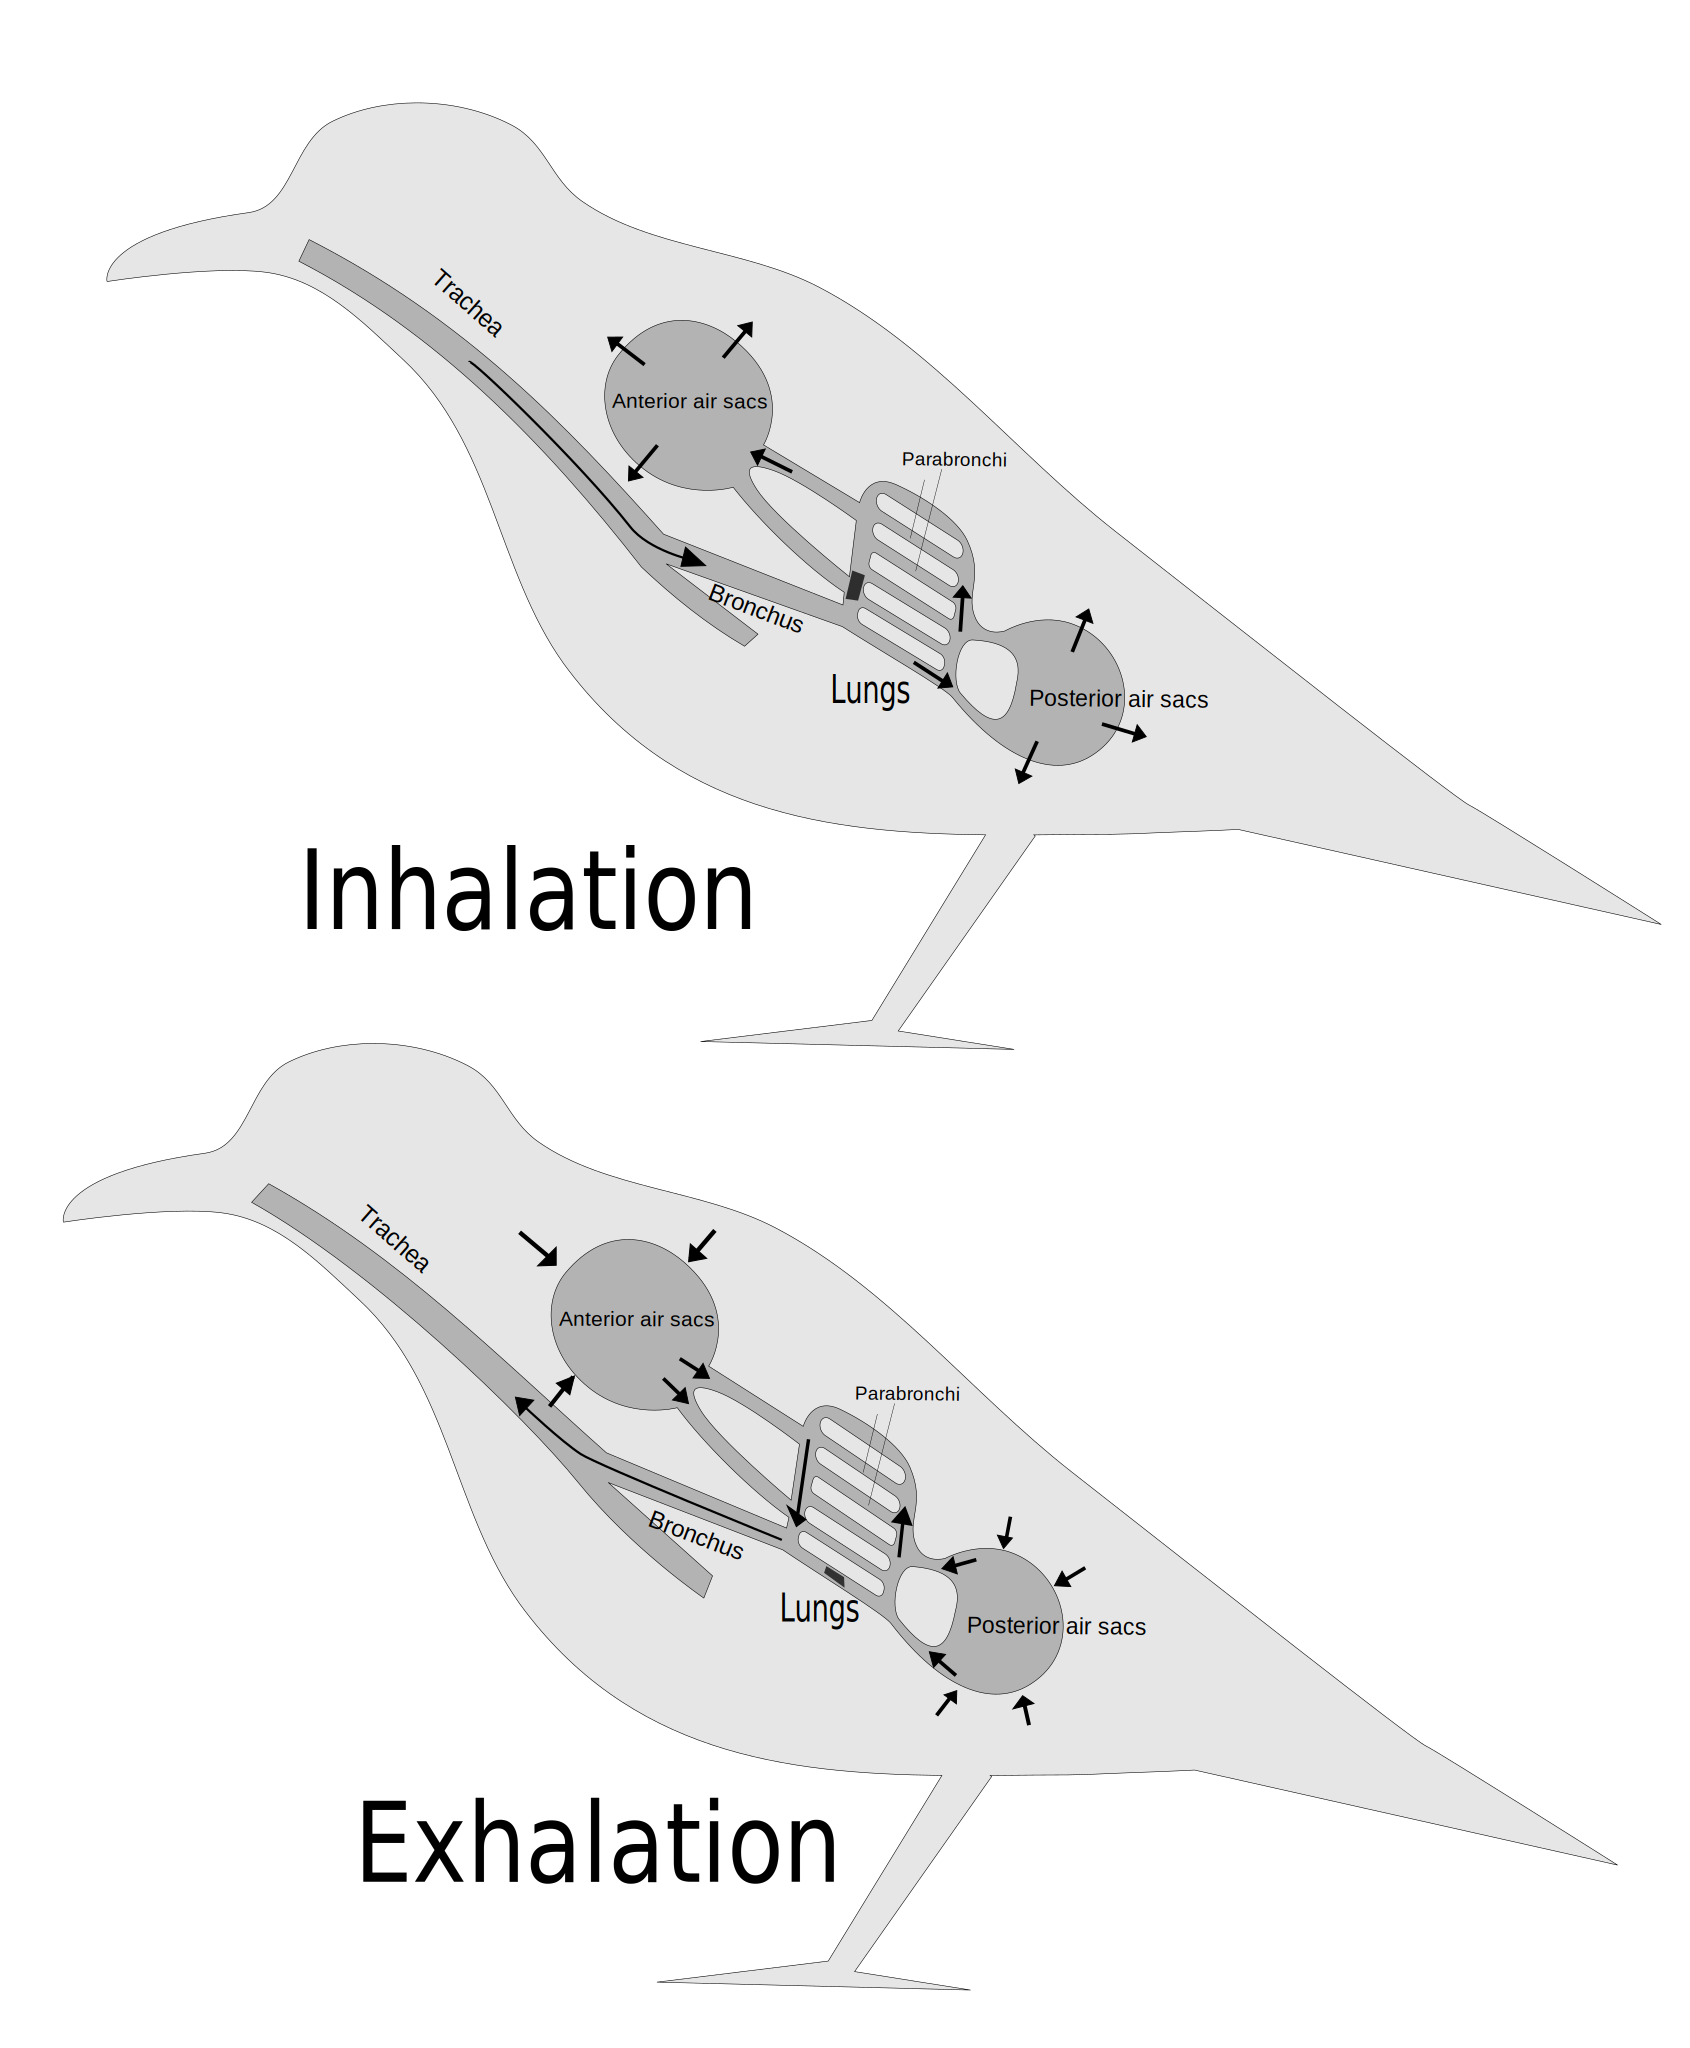
\includegraphics[width=0.7\linewidth]{./figures/respiratory/BirdRespiration} 

}

\caption{\href{https://commons.wikimedia.org/wiki/File:BirdRespiration.svg}{The respiratory system of birds.} On inhalation, air travels to air sacs near the back of a bird. The air then passes through the lungs to air sacs near the front of the bird, from where the air is exhaled.}\label{fig:birdrespiration}
\end{figure}

During inhalation, environmental air initially enters the bird through the nostrils from where it is heated, humidified, and filtered in the nasal passages and upper parts of the trachea. From there, the air enters the lower trachea and continues to just beyond the syrinx, at which point the trachea branches into two primary bronchi, going to the two lungs. The primary bronchi enter the lungs to become the intrapulmonary bronchi, which give off a set of parallel branches called ventrobronchi and, a little further on, an equivalent set of dorsobronchi. The ends of the intrapulmonary bronchi discharge air into the posterior air sacs at the caudal end of the bird. Each pair of dorso-ventrobronchi is connected by a large number of parallel microscopic air capillaries (or parabronchi) where gas exchange occurs. As the bird inhales, tracheal air flows through the intrapulmonary bronchi into the posterior air sacs, as well as into the dorsobronchi (but not into the ventrobronchi whose openings into the intrapulmonary bronchi were previously believed to be tightly closed during inhalation. However, more recent studies have shown that the aerodynamics of the bronchial architecture directs the inhaled air away from the openings of the ventrobronchi, into the continuation of the intrapulmonary bronchus towards the dorsobronchi and posterior air sacs). From the dorsobronchi the air flows through the parabronchi (and therefore the gas exchanger) to the ventrobronchi from where the air can only escape into the expanding anterior air sacs. So, during inhalation, both the posterior and anterior air sacs expand, the posterior air sacs filling with fresh inhaled air, while the anterior air sacs fill with ``spent'' (oxygen-poor) air that has just passed through the lungs.

During exhalation the intrapulmonary bronchi were believed to be tightly constricted between the region where the ventrobronchi branch off and the region where the dorsobronchi branch off. But it is now believed that more intricate aerodynamic features have the same effect. The contracting posterior air sacs can therefore only empty into the dorsobronchi. From there the fresh air from the posterior air sacs flows through the parabronchi (in the same direction as occurred during inhalation) into ventrobronchi. The air passages connecting the ventrobronchi and anterior air sacs to the intrapulmonary bronchi open up during exhalation, thus allowing oxygen-poor air from these two organs to escape via the trachea to the exterior. Oxygenated air therefore flows constantly (during the entire breathing cycle) in a single direction through the parabronchi.

The cross-current respiratory gas exchanger in the lungs of birds. Air is forced from the air sacs unidirectionally (from right to left in the diagram) through the parabronchi. The pulmonary capillaries surround the parabronchi in the manner shown (blood flowing from below the parabronchus to above it in the diagram). Blood or air with a high oxygen content is shown in red; oxygen-poor air or blood is shown in various shades of purple-blue.
The blood flow through the bird lung is at right angles to the flow of air through the parabronchi, forming a cross-current flow exchange system (see illustration on the left). The partial pressure of oxygen in the parabronchi declines along their lengths as O\textsubscript{2} diffuses into the blood. The blood capillaries leaving the exchanger near the entrance of airflow take up more O\textsubscript{2} than do the capillaries leaving near the exit end of the parabronchi. When the contents of all capillaries mix, the final partial pressure of oxygen of the mixed pulmonary venous blood is higher than that of the exhaled air, but is nevertheless less than half that of the inhaled air, thus achieving roughly the same systemic arterial blood partial pressure of oxygen as mammals do with their bellows-type lungs.

The trachea is an area of dead space: the oxygen-poor air it contains at the end of exhalation is the first air to re-enter the posterior air sacs and lungs. In comparison to the mammalian respiratory tract, the dead space volume in a bird is, on average, 4.5 times greater than it is in mammals of the same size. Birds with long necks will inevitably have long tracheae, and must therefore take deeper breaths than mammals do to make allowances for their greater dead space volumes. In some birds (e.g.~the whooper swan, Cygnus cygnus, the white spoonbill, Platalea leucorodia, the whooping crane, Grus americana, and the helmeted curassow, Pauxi pauxi) the trachea, which some cranes can be 1.5 m long, is coiled back and forth within the body, drastically increasing the dead space ventilation. The purpose of this extraordinary feature is unknown.

Air passes unidirectionally through the lungs during both exhalation and inspiration, causing, except for the oxygen-poor dead space air left in the trachea after exhalation and breathed in at the beginning of inhalation, little to no mixing of new oxygen-rich air with spent oxygen-poor air (as occurs in mammalian lungs), changing only (from oxygen-rich to oxygen-poor) as it moves (unidirectionally) through the parabronchi.

Avian lungs do not have alveoli as mammalian lungs do. Instead they contain millions of narrow passages known as parabronchi, connecting the dorsobronchi to the ventrobronchi at either ends of the lungs. Air flows anteriorly (caudal to cranial) through the parallel parabronchi. These parabronchi have honeycombed walls. The cells of the honeycomb are dead-end air vesicles, called atria, which project radially from the parabronchi. The atria are the site of gas exchange by simple diffusion. The blood flow around the parabronchi (and their atria), forms a cross-current gas exchanger (see diagram on the left).

All species of birds with the exception of the penguin, have a small region of their lungs devoted to ``neopulmonic parabronchi''. This unorganized network of microscopic tubes branches off from the posterior air sacs, and open haphazardly into both the dorso- and ventrobronchi, as well as directly into the intrapulmonary bronchi. Unlike the parabronchi, in which the air moves unidirectionally, the air flow in the neopulmonic parabronchi is bidirectional. The neopulmonic parabronchi never make up more than 25\% of the total gas exchange surface of birds.

The syrinx is the sound-producing vocal organ of birds, located at the base of a bird's trachea. As with the mammalian larynx, sound is produced by the vibration of air flowing across the organ. The syrinx enables some species of birds to produce extremely complex vocalizations, even mimicking human speech. In some songbirds, the syrinx can produce more than one sound at a time.

\hypertarget{the-respiratory-system-of-reptiles}{%
\section{The Respiratory System of Reptiles}\label{the-respiratory-system-of-reptiles}}

The anatomical structure of the lungs is less complex in reptiles than in mammals, with reptiles lacking the very extensive airway tree structure found in mammalian lungs. Gas exchange in reptiles still occurs in alveoli however. Reptiles do not possess a diaphragm. Thus, breathing occurs via a change in the volume of the body cavity which is controlled by contraction of intercostal muscles in all reptiles except turtles. In turtles, contraction of specific pairs of flank muscles governs inhalation and exhalation.

\hypertarget{the-respiratory-system-of-amphibians}{%
\section{The Respiratory System of Amphibians}\label{the-respiratory-system-of-amphibians}}

Both the lungs and the skin serve as respiratory organs in amphibians. The ventilation of the lungs in amphibians relies on positive pressure ventilation. Muscles lower the floor of the oral cavity, enlarging it and drawing in air through the nostrils into the oral cavity. With the nostrils and mouth closed, the floor of the oral cavity is then pushed up, which forces air down the trachea into the lungs. The skin of these animals is highly vascularized and moist, with moisture maintained via secretion of mucus from specialised cells, and is involved in cutaneous respiration. While the lungs are of primary organs for gas exchange between the blood and the environmental air (when out of the water), the skin's unique properties aid rapid gas exchange when amphibians are submerged in oxygen-rich water. Some amphibians have gills, either in the early stages of their development (e.g.~tadpoles of frogs), while others retain them into adulthood (e.g.~some salamanders).



\begin{figure}

{\centering 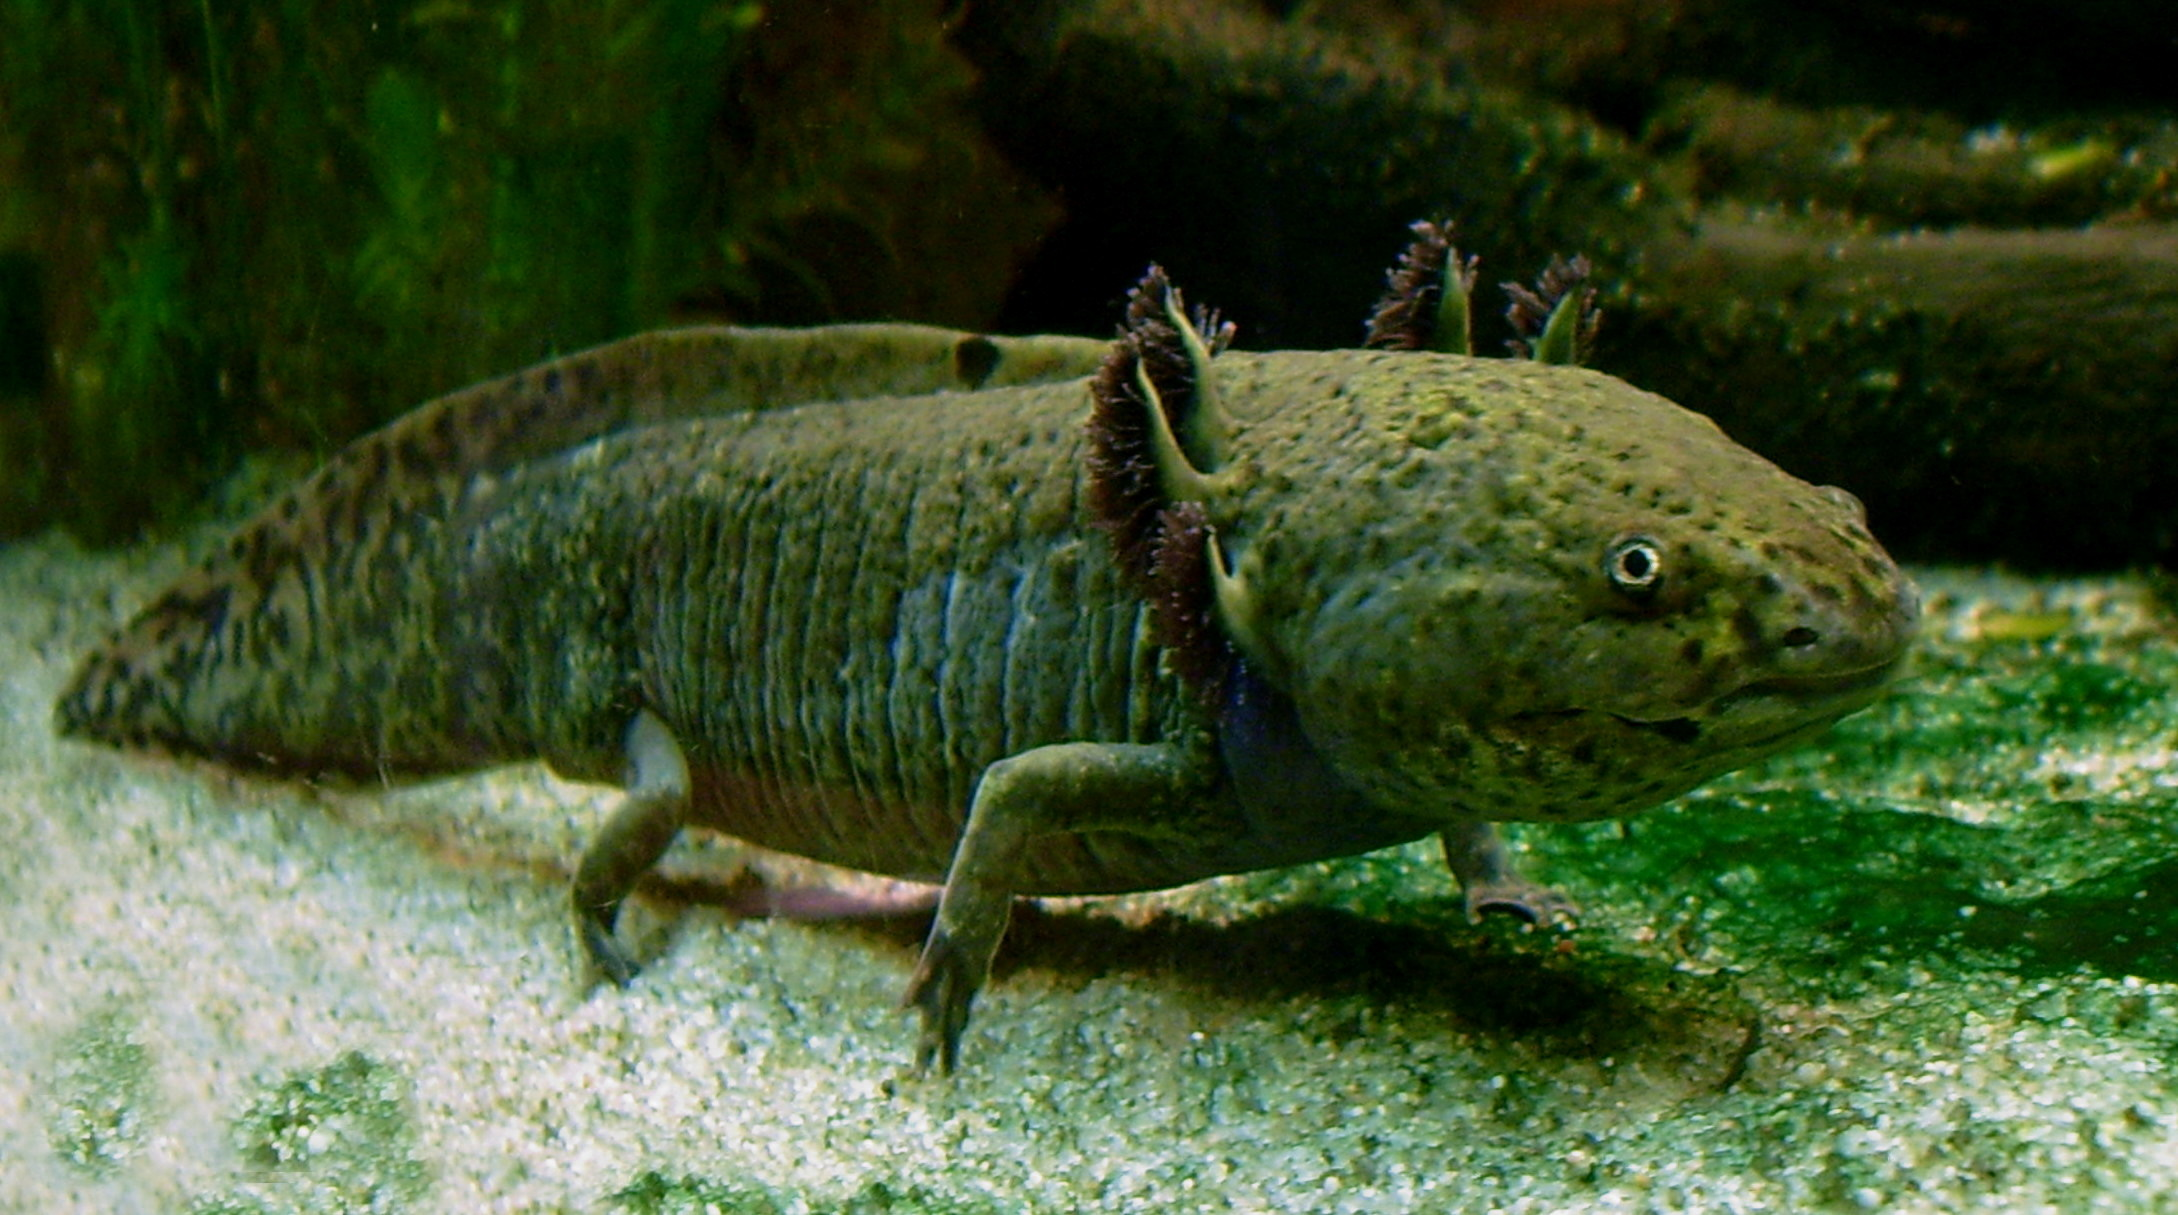
\includegraphics[width=0.7\linewidth]{./figures/respiratory/Axolotl_ganz} 

}

\caption{\href{https://commons.wikimedia.org/wiki/File:Axolotl_ganz.jpg}{The axolotl (\emph{Ambystoma mexicanum}) retains its larval form with gills into adulthood.}}\label{fig:axolotl}
\end{figure}

\hypertarget{the-respiratory-system-of-fish}{%
\section{The Respiratory System of Fish}\label{the-respiratory-system-of-fish}}

Oxygen is poorly soluble in water. Fully aerated fresh water therefore contains only 8--10 ml O\textsubscript{2})/liter compared to the O\textsubscript{2}) concentration of 210 ml/liter in the air at sea level. Furthermore, the coefficient of diffusion (i.e.~the rate at which a substances diffuses from a region of high concentration to one of low concentration, under standard conditions) of the respiratory gases is typically 10,000 faster in air than in water. Thus oxygen, for instance, has a diffusion coefficient of 17.6 mm2/s in air, but only 0.0021 mm2/s in water. The corresponding values for carbon dioxide are 16 mm2/s in air and 0.0016 mm2/s in water. This means that when oxygen is taken up from the water in contact with a gas exchanger, it is replaced considerably more slowly by the oxygen from the oxygen-rich regions small distances away from the exchanger than would have occurred in air. Fish have developed gills deal with these problems. Gills are specialized organs containing filaments, which further divide into lamellae. The lamellae contain a dense thin walled capillary network that exposes a large gas exchange surface area to the very large volumes of water passing over them.

Gills use a countercurrent exchange system that increases the efficiency of oxygen-uptake from the water. Fresh oxygenated water taken in through the mouth is uninterruptedly ``pumped'' through the gills in one direction, while the blood in the lamellae flows in the opposite direction, creating the countercurrent blood and water flow (Fig. 22), on which the fish's survival depends.

Water is drawn in through the mouth by closing the operculum (gill cover), and enlarging the mouth cavity (Fig. 23). Simultaneously the gill chambers enlarge, producing a lower pressure there than in the mouth causing water to flow over the gills. The mouth cavity then contracts inducing the closure of the passive oral valves, thereby preventing the back-flow of water from the mouth (Fig. 23). The water in the mouth is, instead, forced over the gills, while the gill chambers contract emptying the water they contain through the opercular openings (Fig. 23). Back-flow into the gill chamber during the inhalatory phase is prevented by a membrane along the ventroposterior border of the operculum (diagram on the left in Fig. 23). Thus the mouth cavity and gill chambers act alternately as suction pump and pressure pump to maintain a steady flow of water over the gills in one direction. Since the blood in the lamellar capillaries flows in the opposite direction to that of the water, the consequent countercurrent flow of blood and water maintains steep concentration gradients for oxygen and carbon dioxide along the entire length of each capillary (lower diagram in Fig. 22). Oxygen is, therefore, able to continually diffuse down its gradient into the blood, and the carbon dioxide down its gradient into the water. Although countercurrent exchange systems theoretically allow an almost complete transfer of a respiratory gas from one side of the exchanger to the other, in fish less than 80\% of the oxygen in the water flowing over the gills is generally transferred to the blood.

In certain active pelagic sharks, water passes through the mouth and over the gills while they are moving, in a process known as ``ram ventilation''. While at rest, most sharks pump water over their gills, as most bony fish do, to ensure that oxygenated water continues to flow over their gills. But a small number of species have lost the ability to pump water through their gills and must swim without rest. These species are obligate ram ventilators and would presumably asphyxiate if unable to move. Obligate ram ventilation is also true of some pelagic bony fish species.

There are a few fish that can obtain oxygen for brief periods of time from air swallowed from above the surface of the water. Thus Lungfish possess one or two lungs, and the labyrinth fish have developed a special ``labyrinth organ'', which characterizes this suborder of fish. The labyrinth organ is a much-folded suprabranchial accessory breathing organ. It is formed by a vascularized expansion of the epibranchial bone of the first gill arch, and is used for respiration in air.

This organ allows labyrinth fish to take in oxygen directly from the air, instead of taking it from the water in which they reside through use of gills. The labyrinth organ helps the oxygen in the inhaled air to be absorbed into the bloodstream. As a result, labyrinth fish can survive for a short period of time out of water, as they can inhale the air around them, provided they stay moist.

Labyrinth fish are not born with functional labyrinth organs. The development of the organ is gradual and most juvenile labyrinth fish breathe entirely with their gills and develop the labyrinth organs when they grow older.

\hypertarget{the-respiratory-system-of-arthropods}{%
\section{The Respiratory System of Arthropods}\label{the-respiratory-system-of-arthropods}}

Some species of crab use a respiratory organ called a branchiostegal lung. Its gill-like structure increases the surface area for gas exchange which is more suited to taking oxygen from the air than from water. Some of the smallest spiders and mites can breathe simply by exchanging gas through the surface of the body. Larger spiders, scorpions and other arthropods use a primitive book lung.



\begin{figure}

{\centering 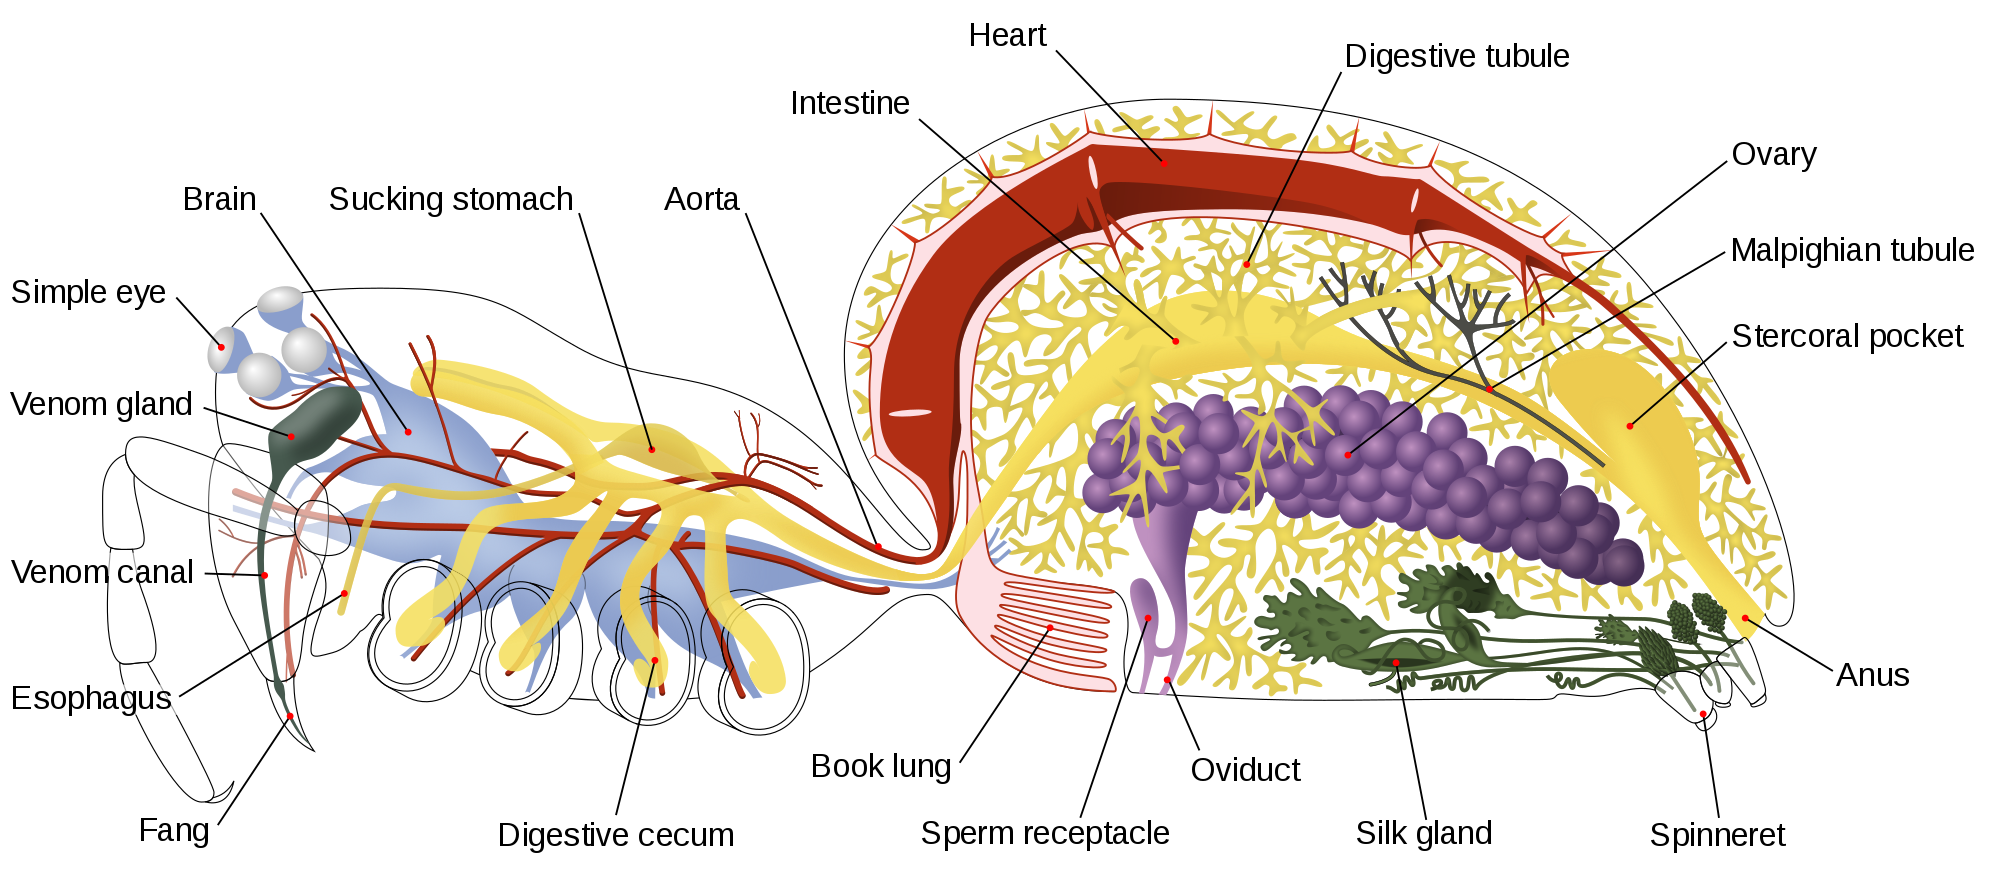
\includegraphics[width=0.7\linewidth]{./figures/respiratory/Spider_internal_anatomy-en} 

}

\caption{\href{https://upload.wikimedia.org/wikipedia/commons/2/22/Spider_internal_anatomy-en.svg}{The book lungs of a spider.}}\label{fig:spiderbooklkung}
\end{figure}

Insects

Most insects breath passively through their spiracles (special openings in the exoskeleton) and the air reaches every part of the body by means of a series of smaller and smaller tubes called `trachaea' when their diameters are relatively large, and `tracheoles' when their diameters are very small. The tracheoles make contact with individual cells throughout the body. They are partially filled with fluid, which can be withdrawn from the individual tracheoles when the tissues, such as muscles, are active and have a high demand for oxygen, bringing the air closer to the active cells. This is probably brought about by the buildup of lactic acid in the active muscles causing an osmotic gradient, moving the water out of the tracheoles and into the active cells. Diffusion of gases is effective over small distances but not over larger ones, this is one of the reasons insects are all relatively small. Insects which do not have spiracles and trachaea, such as some Collembola, breathe directly through their skins, also by diffusion of gases.

The number of spiracles an insect has is variable between species, however, they always come in pairs, one on each side of the body, and usually one pair per segment. Some of the Diplura have eleven, with four pairs on the thorax, but in most of the ancient forms of insects, such as Dragonflies and Grasshoppers there are two thoracic and eight abdominal spiracles. However, in most of the remaining insects, there are fewer. It is at the level of the tracheoles that oxygen is delivered to the cells for respiration.

Insects were once believed to exchange gases with the environment continuously by the simple diffusion of gases into the tracheal system. More recently, however, large variation in insect ventilatory patterns has been documented and insect respiration appears to be highly variable. Some small insects do not demonstrate continuous respiratory movements and may lack muscular control of the spiracles. Others, however, utilize muscular contraction of the abdomen along with coordinated spiracle contraction and relaxation to generate cyclical gas exchange patterns and to reduce water loss into the atmosphere. The most extreme form of these patterns is termed discontinuous gas exchange cycles.

\hypertarget{the-respiratory-system-of-molluscs}{%
\section{The Respiratory System of Molluscs}\label{the-respiratory-system-of-molluscs}}

Molluscs generally possess gills that allow gas exchange between the aqueous environment and their circulatory systems. These animals also possess a heart that pumps blood containing hemocyanin as its oxygen-capturing molecule. Hence, this respiratory system is similar to that of vertebrate fish. The respiratory system of gastropods can include either gills or a lung.

\hypertarget{the-respiratory-system-of-plants}{%
\section{The Respiratory System of Plants}\label{the-respiratory-system-of-plants}}

Plants use carbon dioxide gas in the process of photosynthesis, and exhale oxygen gas as waste. The chemical equation of photosynthesis is 6 CO\textsubscript{2}) (carbon dioxide) and 6 H2) (water), which in the presence of sunlight makes C\textsubscript{6}H\textsubscript{12}O\textsubscript{6} (glucose) and 6 O\textsubscript{2}) (oxygen). Photosynthesis uses electrons on the carbon atoms as the repository for the energy obtained from sunlight. Respiration is the opposite of photosynthesis. It reclaims the energy to power chemical reactions in cells. In so doing the carbon atoms and their electrons are combined with oxygen forming CO\textsubscript{2}) which is easily removed from both the cells and the organism. Plants use both processes, photosynthesis to capture the energy and oxidative metabolism to use it.

Plant respiration is limited by the process of diffusion. Plants take in carbon dioxide through holes, known as stomata, that can open and close on the undersides of their leaves and sometimes other parts of their anatomy. Most plants require some oxygen for catabolic processes (break-down reactions that release energy). But the quantity of O\textsubscript{2}) used per hour is small as they are not involved in activities that require high rates of aerobic metabolism. Their requirement for air, however, is very high as they need CO\textsubscript{2}) for photosynthesis, which constitutes only 0.04\% of the environmental air. Thus, to make 1 g of glucose requires the removal of all the CO\textsubscript{2}) from at least 18.7 liters of air at sea level. But inefficiencies in the photosynthetic process cause considerably greater volumes of air to be used.


